\chapter{Emerging Jets (EJs) \label{ch:emj}}


\section{Background information on EJs}

Although there is a preponderance of evidence from astronomical and cosmological observations for the existence of dark matter \cite{What_is_DM}, it has not yet been detected in laboratories, suggesting that its origin may be associated with as-of-yet unobserved physics processes beyond the Standard Model. As experimental searches have excluded a large portion of the phase space of DM models with weakly interacting massive particles \cite{WIMPS}, alternative theoretical models have been developed with a hidden gauge sector, similar to quantum chromodynamics (QCD), which can result in strongly self-interacting DM particles. Dark matter of his type could interact with SM particles through so-called mediator particles and potentially be produced at colliders, producing signatures such as semivisible jets \cite{Nabili:2886140} or emerging jets\cite{sirunyan2019search}.

The EJ concept is described here in \cite{Schwaller:2015gea}. This was used to look for EJs in the Run 1 dataset of the CMS Experiment.
However, our current Run-2 EJ analysis surpasses the Run-1 search for EJs in the unflavored scenario, increasing the experimental limit of the dark mediator particle by 500 GeV to set the most stringent limits to date, and provides the first direct exclusion of the flavor-aligned scenario.
The EJs model is a dark matter model that assumes that there is a QCD-like hidden sector. In particular, in these high-energy collisions, a heavy dark mediator ($X_{DK}$) is produced with a mass on the $\order{\text{TeV}}$, decaying into dark hadrons and mesons that further decay into SM particles. Due to the hierarchy of GeV to TeV energy scales (see \Cref{fig:dark-qcdmodel}), the decay process allows for dark matter particles to travel a measurable distance before decaying.
In \Cref{fig:emj_production1} we see the production processes of the EJs signature. There are 2 ways of producing EJs in the LHC. First, is through gluon-gluon fusion and second is from quark anti-quark annihilation.
Both of these produce a pair of heavy dark mediators, each then decays into an SM quark (\textit{q}) and a dark quark (\Qdark). Further on, we see from \Cref{fig:full-chain} that the \Qdark will decay into \pidark.
Since these dark pions are unstable and do not carry a dark baryon number, they then decay after some measurable distance into SM particles \cite{Bai_2014} and form SM jets that we can detect.


\begin{figure}
	\centering
	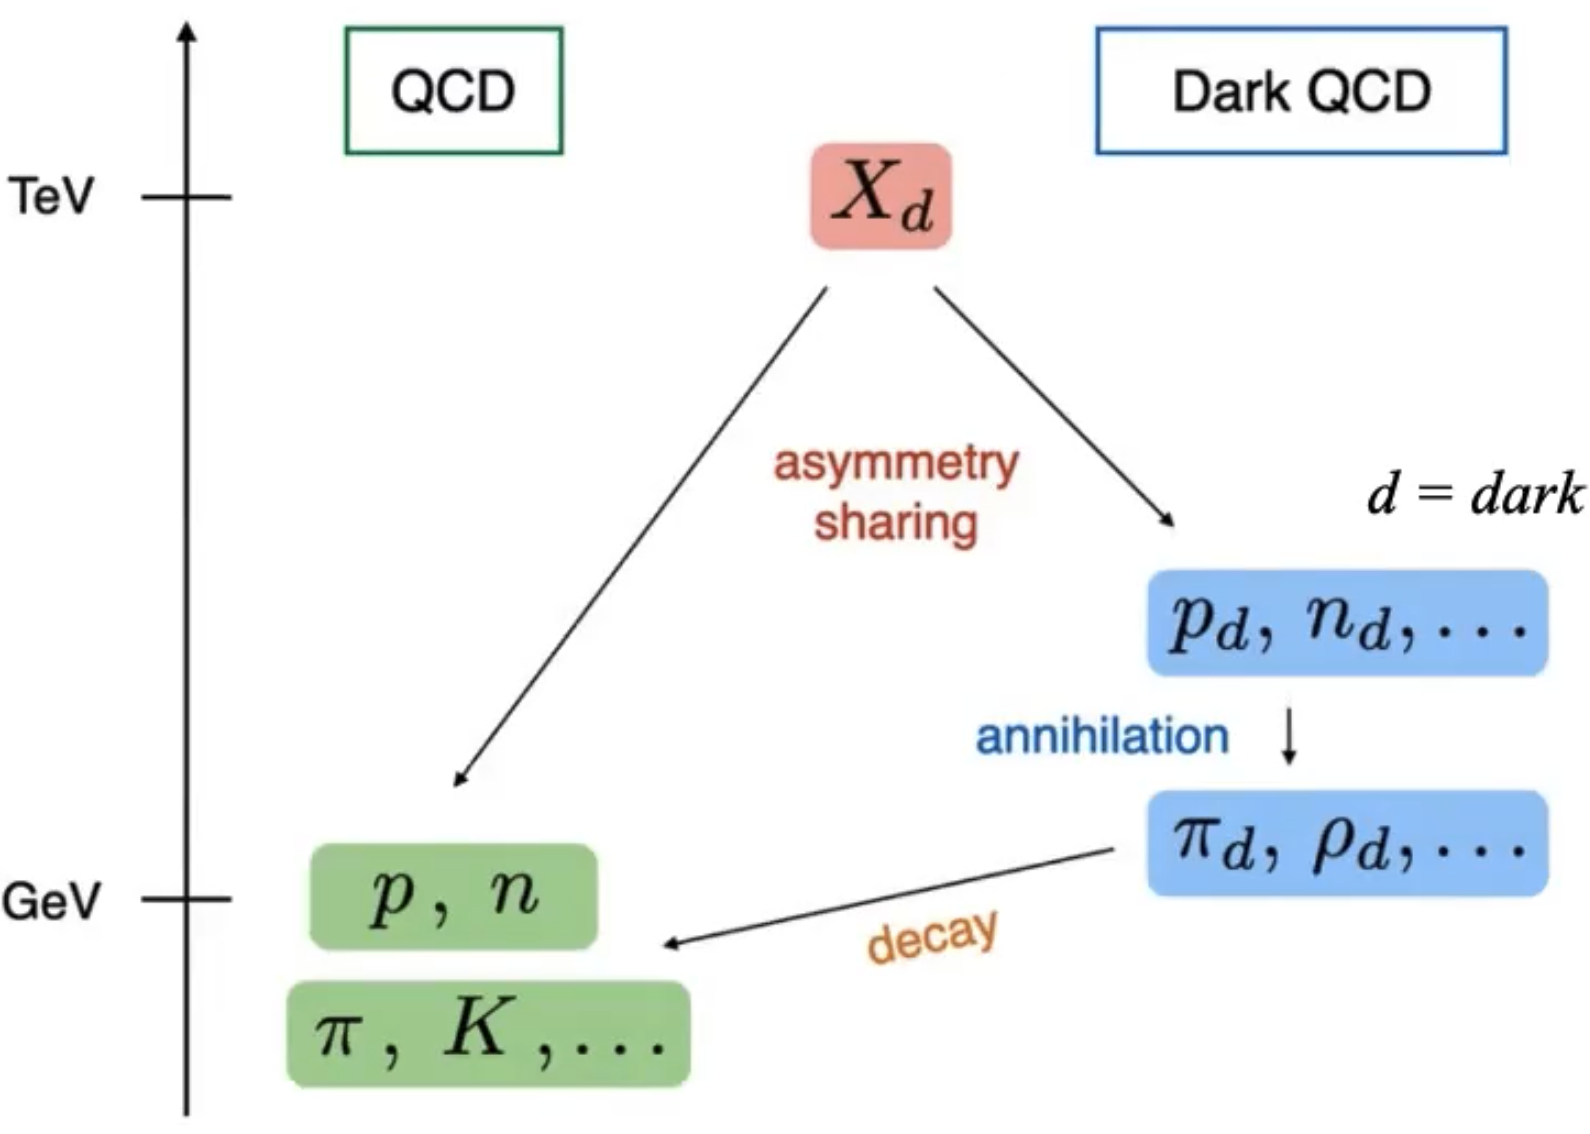
\includegraphics[width=0.8\linewidth]{Images/DarkQCDModel.png}
	\caption[The hierarchy of the GeV to TeV scales.]{The hierarchy of the GeV to TeV scales. In this model the dark scalar mediator $X_d$ couples to both dark and SM sectors. Reprinted from \cite{Schwaller:2015gea}}
	\label{fig:dark-qcdmodel}
\end{figure}


\begin{figure}
	\begin{center}
		\begin{subfigure}{.45\linewidth}
			\includegraphics*[width=\linewidth]{pdfs/BSSWPairProduction_ggFusion.pdf}
			\caption{gluon-gluon fusion}
		\end{subfigure}
		\begin{subfigure}{.45\linewidth}
			\includegraphics*[width=\linewidth]{pdfs/BSSWPairProduction_qqAnnihilation.pdf}
			\caption{quark anti-quark annihilation}
		\end{subfigure}
	\end{center}
	\caption[Emergin jets production modes]{Feynman diagrams for pair production of dark mediator particles, with mediators decay to an SM quark and a dark quark. The bar ($-$) over the quark symbols signify that they are anti-particles, as is the dagger ($\dagger$) over the \Mdark. Taken from internal communications.}
	\label{fig:emj_production1}
\end{figure}

\begin{figure}
	\centering
	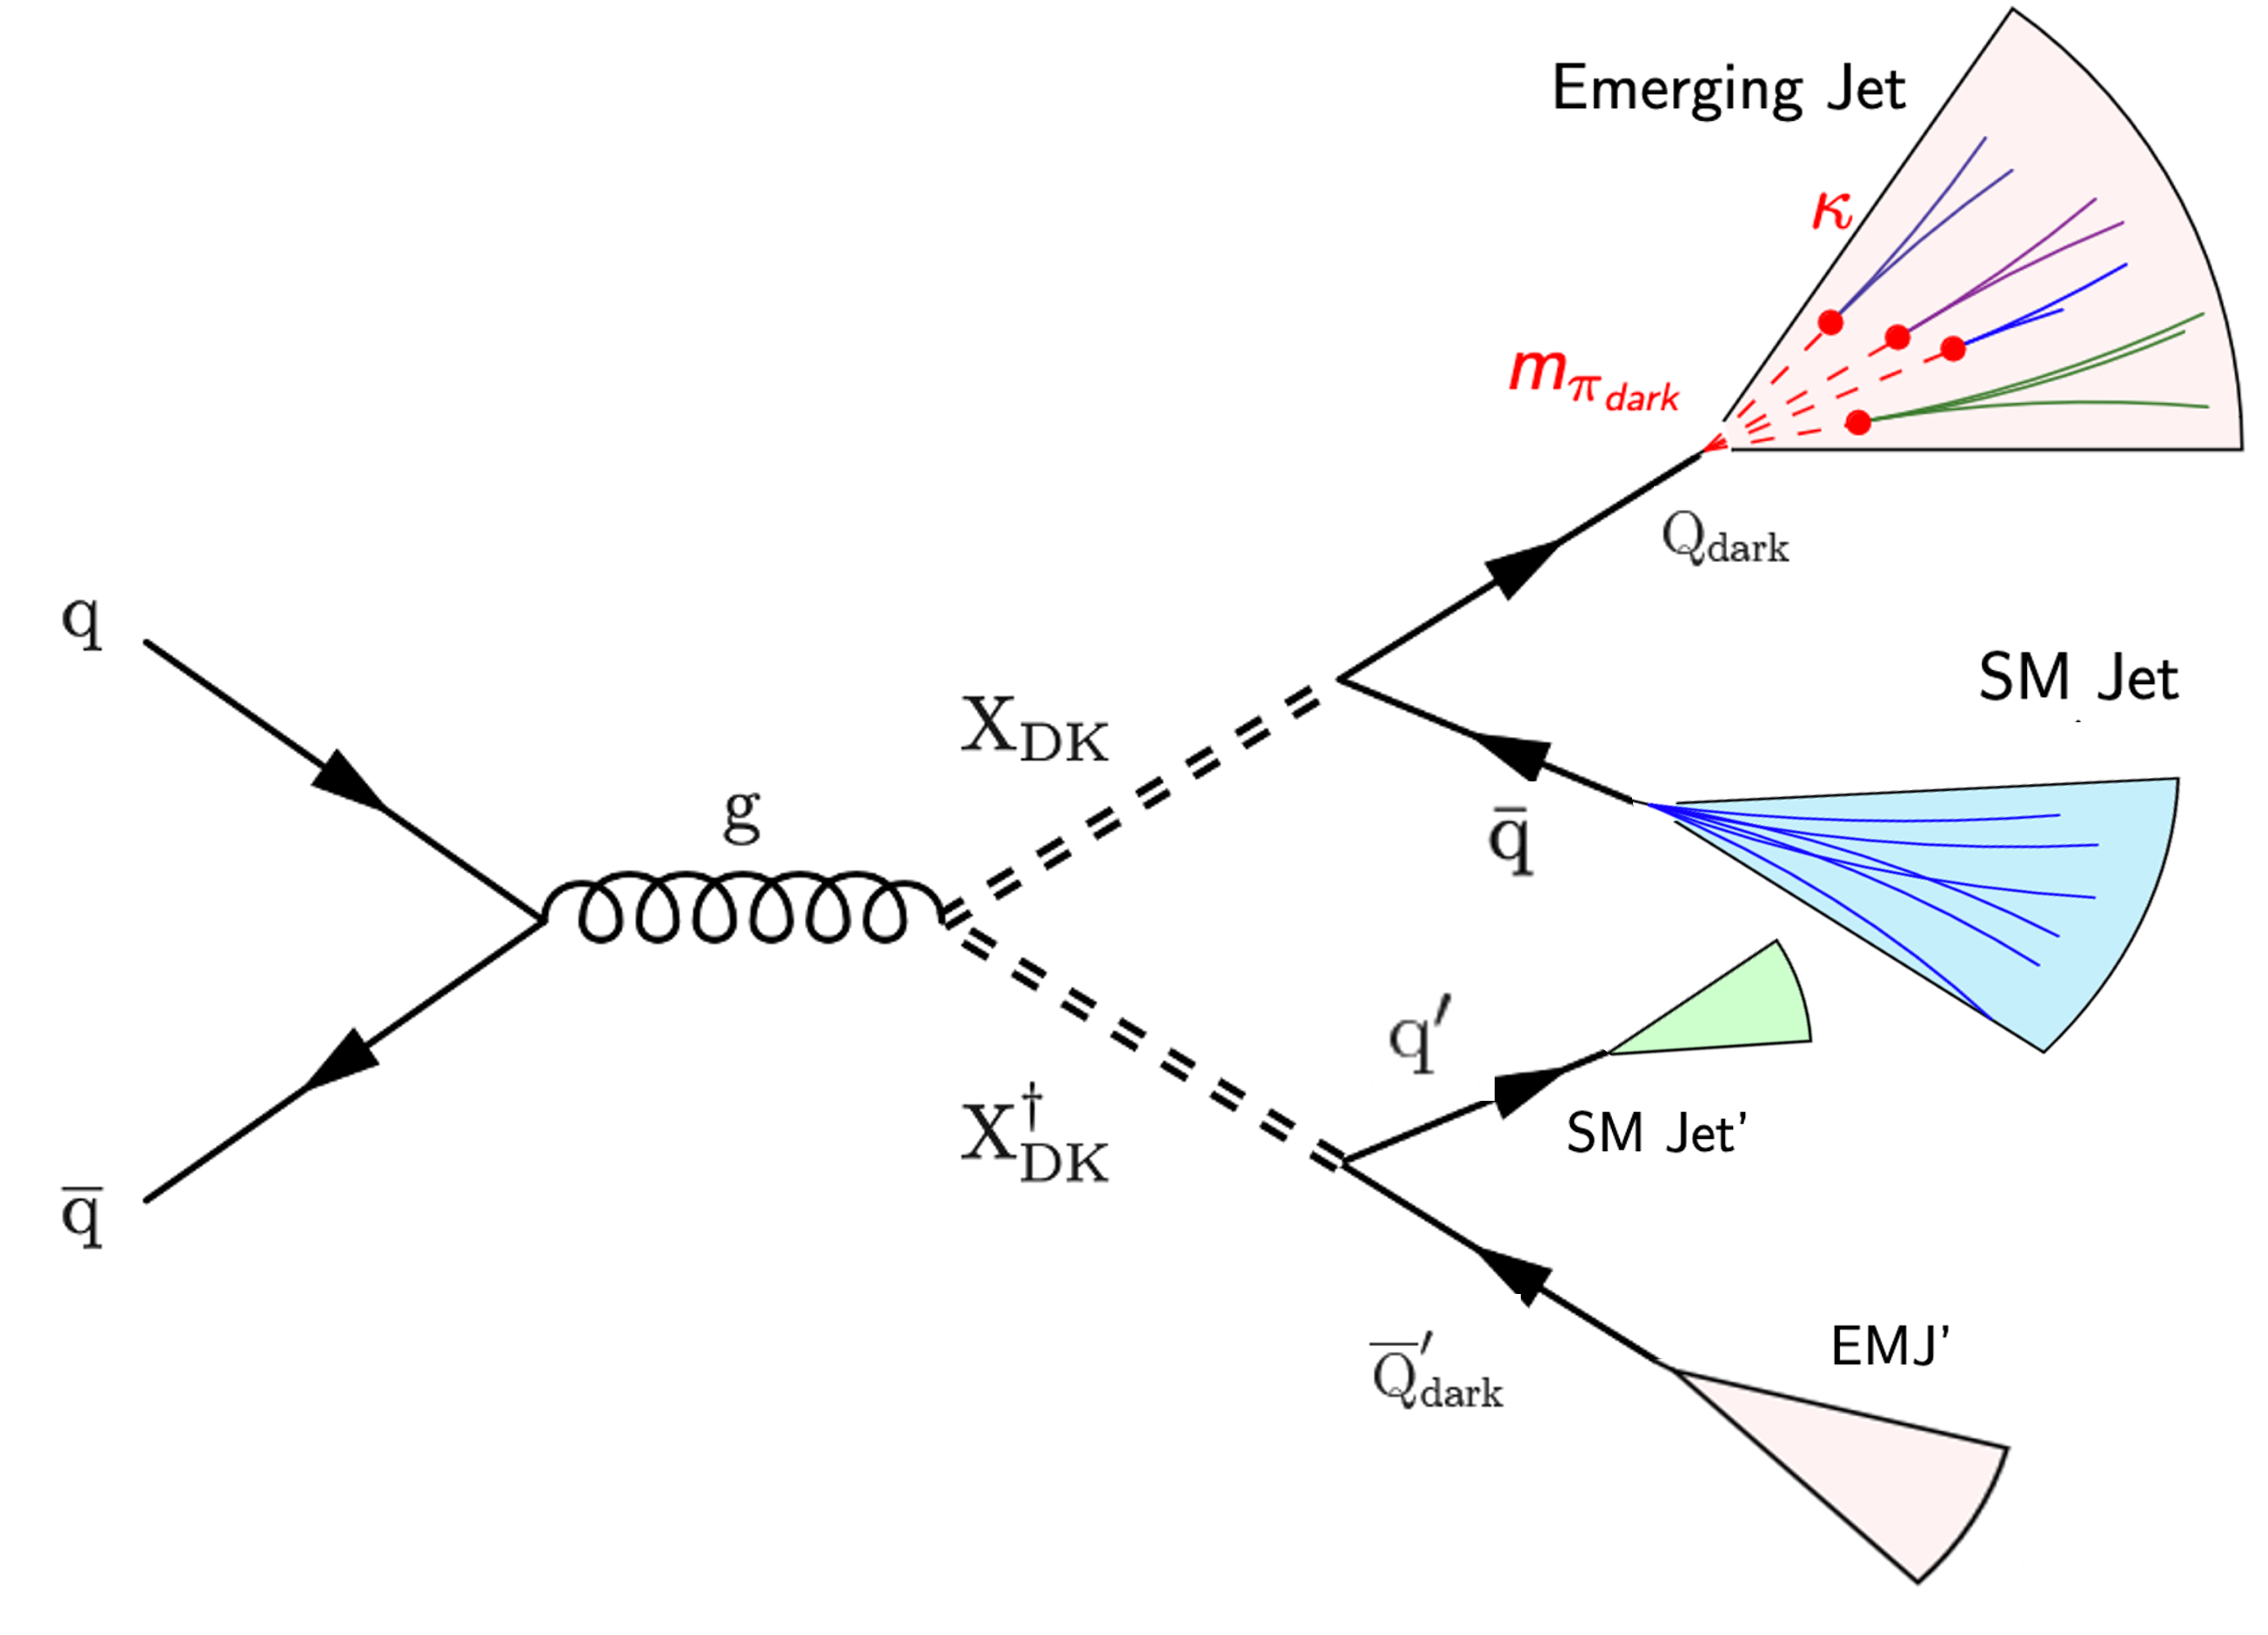
\includegraphics[width=.8\linewidth]{Images/EMJ_production.png}
	\caption{Example of the full chain of one production mode. Taken from internal communications.}
	\label{fig:full-chain}
\end{figure}

\begin{figure}
	\centering
	\begin{subfigure}{.45\linewidth}
		\includegraphics*[width=\textwidth]{pdfs/FlavoredSchematicOfEvent.pdf}
		\caption{Flavor aligned}
		\label{fig:emj_prod2A}
	\end{subfigure}
	\begin{subfigure}{.45\linewidth}
		\includegraphics*[width=\textwidth]{pdfs/UnflavoredSchematicOfEvent.pdf}
		\caption{Unflavored}
	\end{subfigure}
	\caption[Shorter version of the production modes for the Emerging Jets models.]{Shorter version of the production modes for the Emerging Jets models. On the left, we show the flavor-aligned model where all \Qdark couple to down-type SM quarks only (d,s,b).
		This model has \pidark variable lifetimes (\ctaudpi ) which depend on their composition and the Yukawa coupling constant ($\kappa$) between the mediator particle, the dark quarks, and the SM down quark. This parameter represents the lifetime of each track inside emerging jets.
		On the right, we show the simpler unflavored model. This produces \Qdark that couple to the down-quark only and all \pidark lifetimes are the same. Taken from internal communications.}
	\label{fig:emj_production2}
\end{figure}


% Add explanation on two EMJ models
In the experimental searches \cite{sirunyan2019search,CMS:2024gxp} the TeV scale has been explored searching for the EJs signature.
In the latest search, there were 3 free parameters studied. The mediator mass $m_{\Mdark}$ was varied $\in [1,2.5]$ TeV, the dark pion mass $m_{\pidark}\leq 20$ GeV and the dark pion lifetime $\ctaudpi \leq 500$ mm.
The full Run 2 dataset is used in the latest search for emerging jets using the data collected by the CMS Collaboration in 2016--2018 using proton-proton collisions at a center-of-mass energy of 13 TeV accumulating 138~\unit{\per\femto\barn} worth of data \cite{CMS:2024gxp}.
We studied the models described in \cite{Bai_2014,Schwaller:2015gea,Renner_2018} from which we expanded on the phase space searched in \cite{sirunyan2019search} and included the flavored model portrayed in \Cref{fig:emj_prod2A} that allows for the \Qdark to couple to all down-type quarks. In this model, each dark sub-component (or \pidark) within the dark jet can subsequently decay into standard model particles at different distances along the jet axis.
Here, lifetimes for the dark mesons are dependent on the \Qdark composition and the Yukawa coupling constant ($\kappa$) between the dark quarks and the SM down quark.
In the unflavored model, all \Qdark are degenerate, while in the flavored model, three dark quark flavors with non-degenerate couplings are considered.
For the unflavored model, the average decay length of a dark pion is given by \Cref{eq:unflavored-ctau}
\begin{equation}
	\ctaudpi = 80~\unit{mm} \pgroup{\frac{1}{\kappa^4}} \pgroup{\frac{2 ~\unit{GeV} }{f_{\pidark}}}^2 \pgroup{\frac{100 ~\unit{MeV}}{m_\text{d}} }^2 \pgroup{\frac{2~\unit{GeV}}{m_{\pidark}}} \pgroup{\frac{m_{\Mdark}}{1~\unit{TeV}}}^4
	\label{eq:unflavored-ctau}
\end{equation}
where $f_{\pidark}$ is the dark pion decay constant, $m_\text{d}$ is the mass of the SM down quark, and $m_{\pidark}$ is the dark pion mass. In the flavored aligned model, the coupling constant is now a matrix $\kappa_{\alpha i}$ where the subscript $\alpha ~(i)$ denotes flavors of dark (SM) quarks. In this case, the average decay length for dark mesons is given by \Cref{eq:flavored-ctau}
\begin{equation}
	\small
	\ctaudpi^{\alpha \beta} = \dfrac{8\pi m^4_{\Mdark}}{ N_c m_{\pidark} f^2_{\pidark} \displaystyle \sum_{i,j} \abs{\kappa_{\alpha i} \kappa_{\beta j}^*}^2 \pgroup{m_i^2 + m_j^2} \sqrt{ \pgroup{1- \dfrac{(m_i^2 + m_j^2)^2 }{m^2_{\pidark}} } \pgroup{1- \dfrac{(m_i^2 - m_j^2)^2 }{m^2_{\pidark}} } } }
	\label{eq:flavored-ctau}
\end{equation}
where $m_{\Mdark}$ is the mediator mass, $N_c$ is the SM color factor and $m_i, m_j$ are the masses of the SM quarks with flavor indices $i, j$, respectively\cite{CMS:2024gxp}.
\Cref{fig:lifetimes} shows the different $c\tau$ for a given $m_{\pidark}$ based on the \pidark composition in the flavor-aligned model. In general, the lifetime of the dark pions goes down as their mass increases, as opposed to the unflavored model where the lifetimes are the same for all \pidark.
\begin{figure}[b]
	\centering
	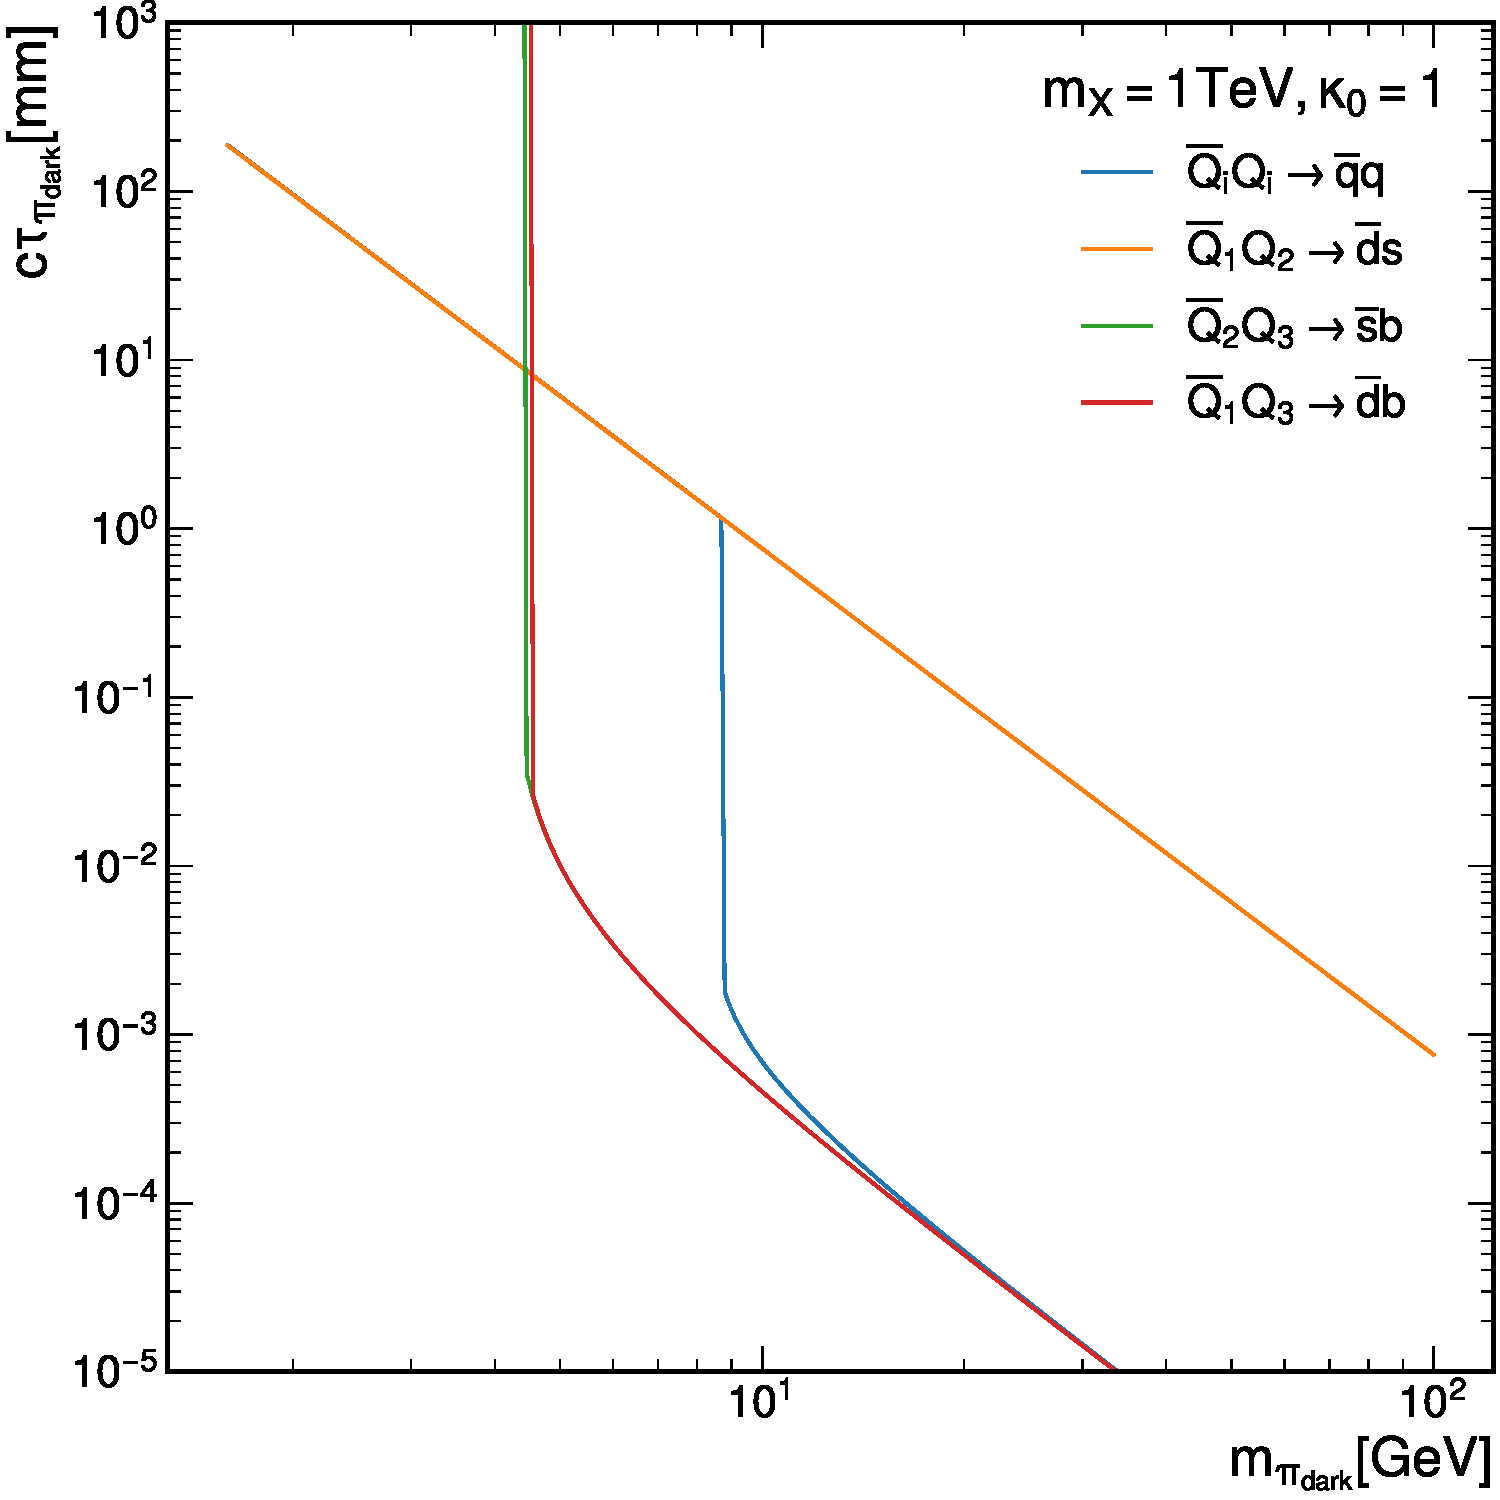
\includegraphics[width=.65\linewidth]{Images/pdfs/FlavoredLifetime.pdf}
	\caption[Lifetimes of the dark pions as a function of their mass.]{Lifetime of the \pidark as a function of the $m_{\pidark}$ in the flavor-aligned model. The jumps in the plot are indications of new energy states becoming available.}
	\label{fig:lifetimes}
\end{figure}

We can see from \Cref{fig:decay-distance} that this model has some distribution of the decay lengths in the order $\order{\unit{mm} - \unit{m}}$. The CMS detector is hence, sensitive to this phenomenon.
\Cref{fig:2emj_inCMS} illustrates how two EJs would look in a detector. It is assumed that from the high-energy collisions, dark quarks with enough energy hadronize and decay into (\pidark). In the detector the SM quarks hadronize to produce SM jets and the dark quarks would also hadronize to make dark jets. The main signature for the analysis is to look for events that have high event energy, in particular in the form of a quantity known as $H_T$. The $H_T$ of an event is defined as the scalar sum of the transverse momentum ($\Vec{p}_T$) of the 4 leading jets (2 EJs, 2 SM jets).
\begin{equation}
	H_T = \sum_{i=1}^4 p_T^i
\end{equation}

\begin{figure}
	\centering
	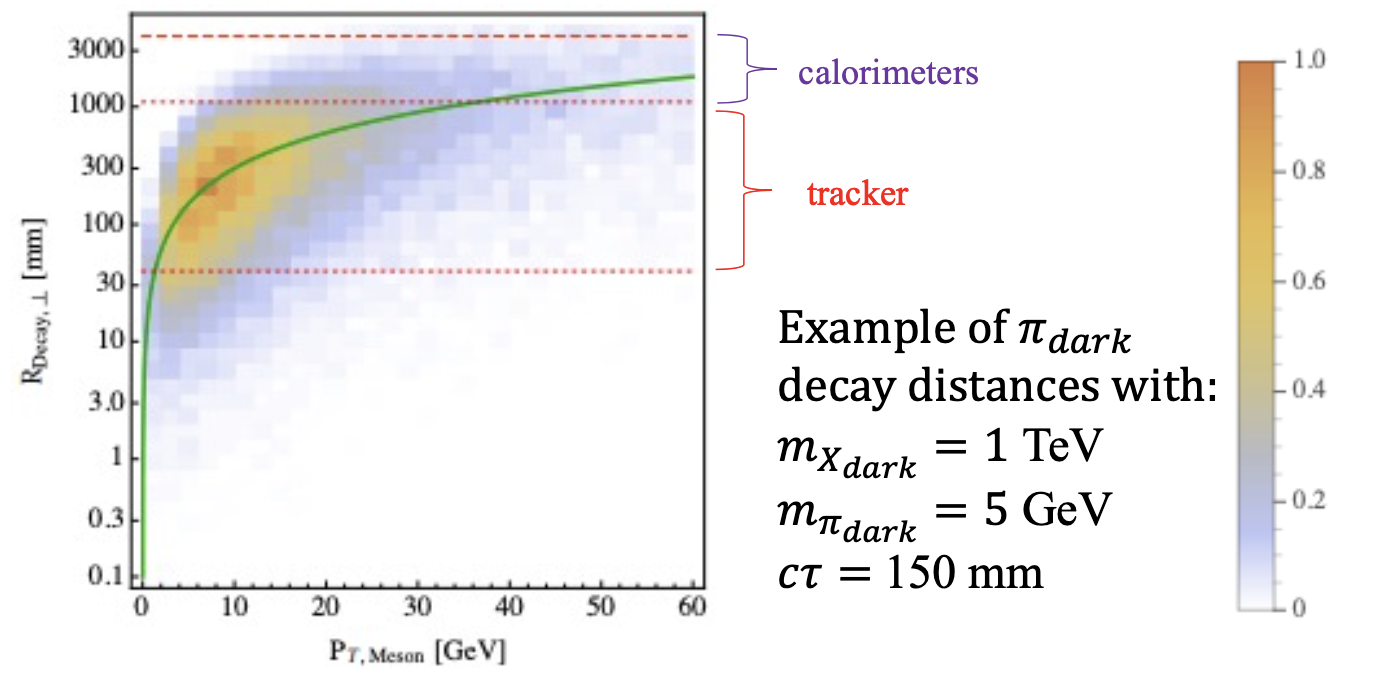
\includegraphics[width=.75\linewidth]{Images/Decay-distances-emj.png}
	\caption[2D distributions of decay distances and $\pi_{DK}$ momentum]{2D distribution between the decay distances and the $\pi_{DK}$ momentum. Reprinted from \cite{Schwaller:2015gea}}
	\label{fig:decay-distance}
\end{figure}

% \begin{itemize}
%     \item $m_{\Mdark} \in [1,2.5]$ TeV
%     \item $m_{\pidark} \leq 20$ GeV
%     \item $\ctaudpi \leq 500$ mm
% \end{itemize}


\begin{figure}
	\centering
	\includegraphics[width=.58\linewidth]{emj_detector.png}
	\caption[Illustration of the emerging jets forming in a detector]{An illustration of the pair production of dark quarks forming two emerging jets. Dashed lines represent the dark mesons as they do not interact with the detector. After traveling some distance, each dark pion decays into Standard Model particles, creating a small jet represented by solid colored lines. Because of the exponential decay, each set of SM particles originates at a different distance from the interaction point, so the jet slowly emerges into the detector. Figure and description adapted from \cite{Schwaller:2015gea}}
	\label{fig:2emj_inCMS}
\end{figure}

Unfortunately, despite the increased amount of data, and the introduction of machine learning techniques to search for EJs, the results of this analysis found no evidence of the EJs signature and excluded mediator masses up to 1950 (1850) GeV for an unflavored (flavor-aligned) dark QCD model within the upper limit of 95\% statistical confidence level \cite{CMS:2024gxp}.

\clearpage

\section{Trigger Efficiency and Scale Factor studies}


With a beam spacing of 25~\unit{ns}, beam crossings occur in the CMS detector at a rate of 40 million per second 40~\unit{\MHz}.
An additional complication is the approximately $>$25 interactions (``pileup'') that occur with each beam crossing -- thus giving 1 billion events occurring in the CMS detector every second. To extract physics from these interactions it is vital to have fast electronics and good resolution (proton-proton interactions are very messy and produce hundreds or thousands of particle candidates) and, because these events occur far too quickly to all be recorded and would take up vast amounts of disk space to store what are, for the majority, uninteresting events, very precise ``triggering'' is required.

Events of interest are selected using a two-tiered trigger system. The first level (L1), composed of custom hardware processors, uses information from the calorimeters and muon detectors to select events at a rate of around 100~\unit{kHz} within a fixed latency of 4~\unit{\us} \cite{CMS:2020cmk}. The second level, known as the high-level trigger (HLT), consists of a farm of processors running a version of the full event reconstruction software optimized for fast processing and reduces the event rate to around 1~\unit{kHz} before data storage~\cite{CMS:2016ngn}.

There are multiple types of triggers, and each will determine the kind of physics dataset that the data will be classified under. There are a few main datasets used to classify physics data, the ones relevant to the analysis are \emph{JetHT} for 2016-2018 and \emph{SinglePhoton}/\emph{EGamma} for 2016-2017/2018. These are considered to be orthogonal datasets as we do not expect a large overlap of the physics process that take place in them. Each category\footnote{also called a data stream} is comprised of an exhaustive list of ``trigger paths'' that are executed to decide what more specific conditions or subprocesses have taken place to record the events.
The $H_T$ triggers chosen are the triggers with the lowest online $H_T$ threshold that are not pre-scaled. The configurations used for this analysis for the \textit{JetHT} data stream are:

\begin{itemize}
	\item \verb|HLT_PFHT900_v* OR HLT_PFJet450_v*| for 2016. The addition of a jet trigger path in an OR configuration is the recommended path to mitigate an observed inefficiency at high values of $H_T$ caused by the Level-1 trigger firmware issues for 2016.
	\item \verb|HLT_PFHT1050_v*| for 2017 and 2018.
\end{itemize}

The paths used for the \textit{SinglePhoton} data stream are:
\begin{itemize}
	\item \verb|Photon165_HE10_v*| for 2016/2016 HIPM
	\item \verb|Photon200_v*| for 2017/2018
\end{itemize}

We also have a simulation equivalent of these main datasets where we have access to the ground truth (Generator-Level) information of the simulated events, called Monte Carlo (MC) simulations.
Though not directly used to draw the conclusions of the search, SM MC samples are used to develop the analysis strategy. The SM multi-jet MC samples are used as a stand-in for expected background events in the \textit{JetHT} data and are used for event/object selection optimization, closure tests and evaluation of uncertainties. The $\gamma$+jets MC samples are used as a stand-in for the \textit{SinglePhoton} data stream, used for template histogram generation, and are compared with the multi-jet MC to evaluate uncertainties associated with \textit{JetHT}/\textit{SinglePhoton} environment differences\cite{CMS:2024gxp}.


The calculation of the trigger efficiency is carried out by using the orthogonal \verb|HLT_Mu50_v*| trigger as the reference trigger. The offline $H_T$ threshold at which the trigger can be considered to be fully efficient was estimated by fitting the trigger efficiency as a function of $H_T$ to an error function (erf) and an algebraic function ($f$):

\begin{align}
	\text{erf}(H_T ;\ A,B,C) & = \frac A2 \left[1+ \text{erf}\left(\dfrac{H_T - |B|}{C}\right) \right]\label{eq:erf} \\
	f(H_T ;\ A,B,C,D)        & = A \dfrac{\frac{H_T - B}{C}}{1+ \left(\frac{H_T - B}{C}\right)^2} + D \label{eq:alg}
\end{align}

Where \Cref{eq:erf,eq:alg} are modeled after the sigmoid-like functions
\[
	\text{erf}(x) = \frac{2}{\sqrt{\pi}} \int_0^x e^{-t^2} \dd{t}
\]
\[
	f(x)=\frac{x}{1+x^{2}}
\]


The fit result is used to determine the threshold at which the $H_T$ trigger is expected to reach 99\% of their plateau value. This is also to assist in the termination of the offline $H_T$ cut applied to signal event selection, to make sure that signal events are not impacted too much by the trigger turn-on effects. \Cref{fig:HT_efficiencies} shows the trigger efficiency as a function of event $H_T$ evaluated in the 4 data collection eras using the \textit{JetHT} data stream compared with QCD simulation along with an estimate of the trigger plateau value.
More specifically, \Cref{fig:HT_eff_16,fig:HT_eff_16_HIPM,fig:HT_eff_17,fig:HT_eff_18} compare efficiency for \HT trigger as a function of event \HT measured relative to \verb|HLT_Mu50_v*| in data (black) and QCD MC (gray) and fit the algebraic function \textit{f} (line). With the computation of the efficiency at each range of \HT, we can compute the ratio between the \HT in data and MC. The ratio of the trigger efficiency in data vs. that in QCD MC is applied to each signal MC event as an $H_T$-dependent scaling factor, and the difference in the event acceptance of applying the scale factor and applying the scale factors with a shifted statistical uncertainty is treated as its systematic uncertainty.

\begin{figure}
	\centering
	\begin{subfigure}{.45\textwidth}
		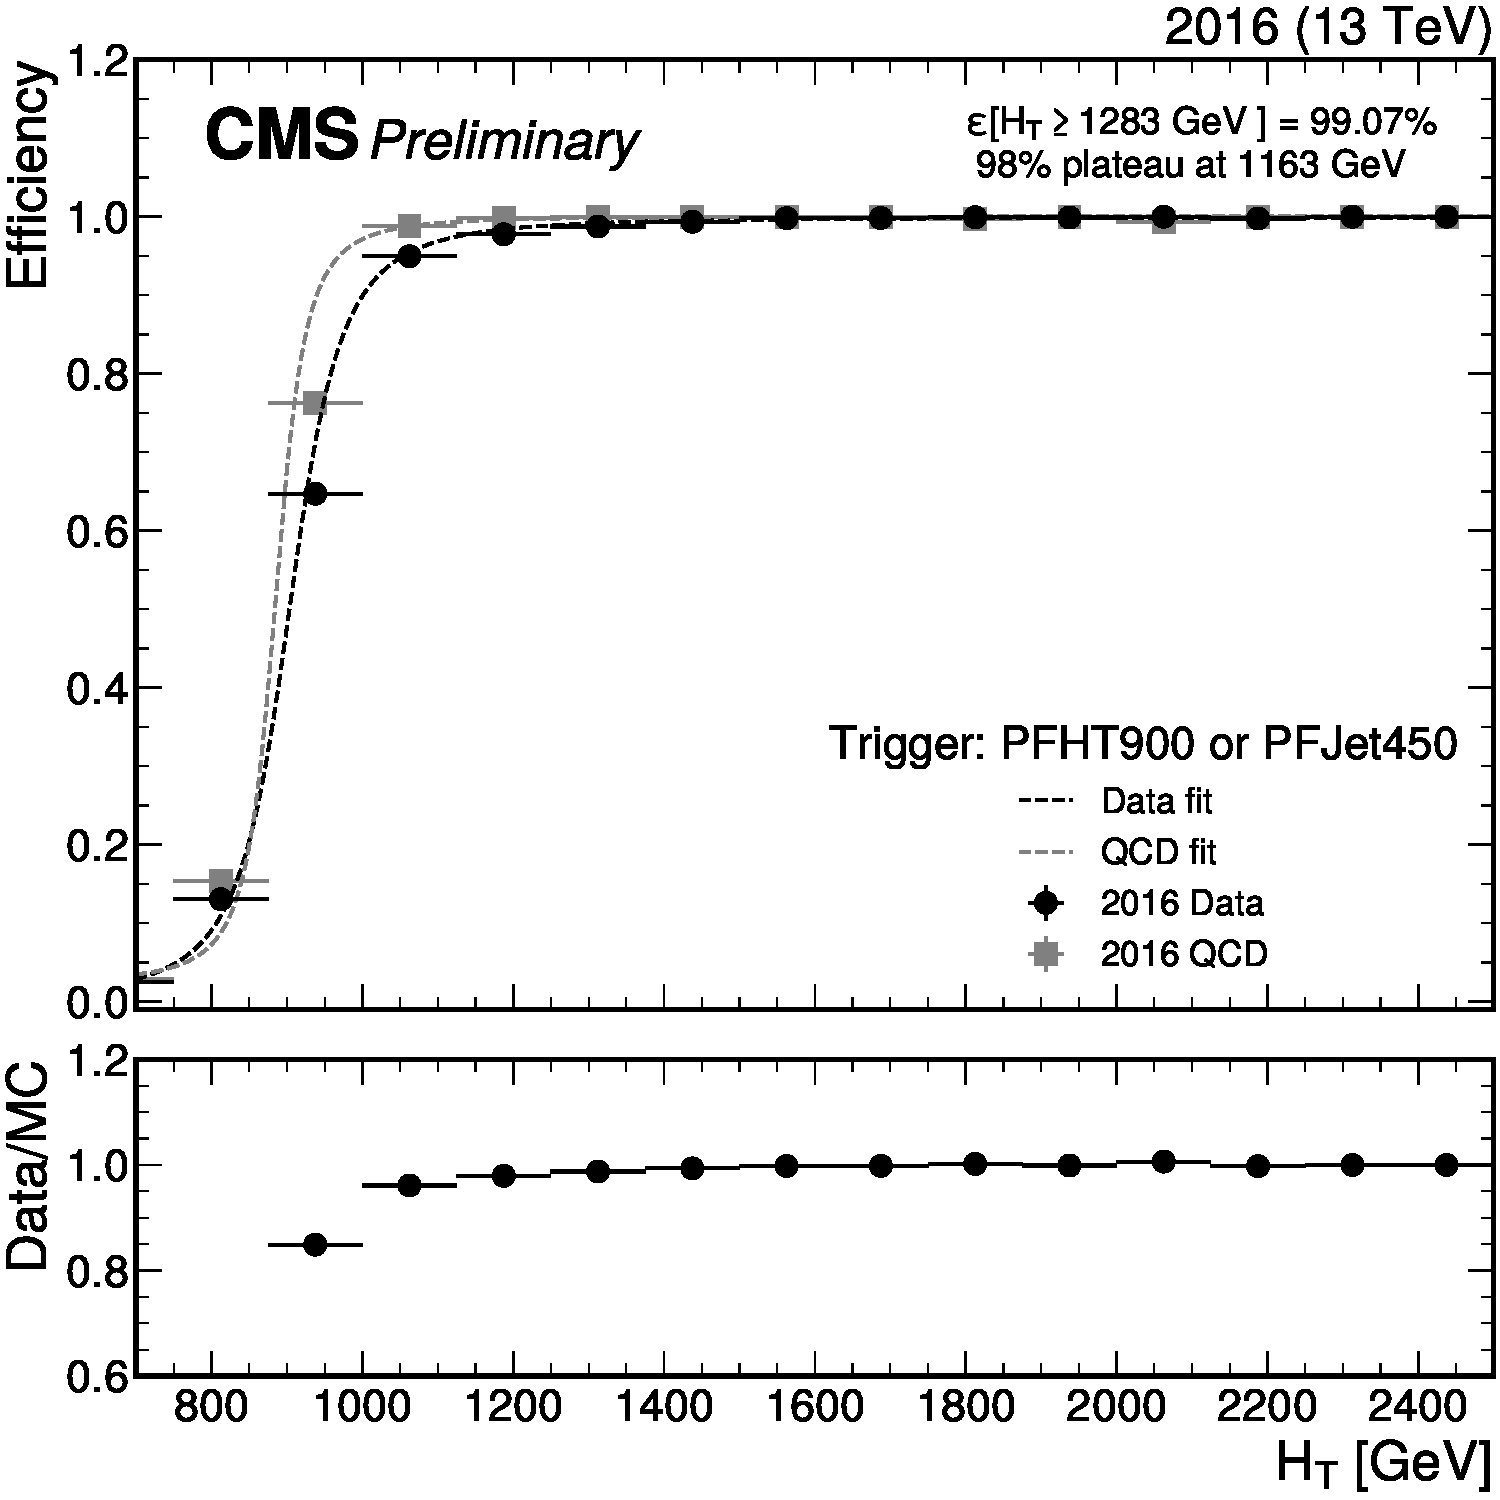
\includegraphics[width=\linewidth]{Images/pdfs/16_efficiency_withratio_and_fits.pdf}
		\caption{Run2 2016}
		\label{fig:HT_eff_16}
	\end{subfigure}
	%
	\begin{subfigure}{.45\textwidth}
		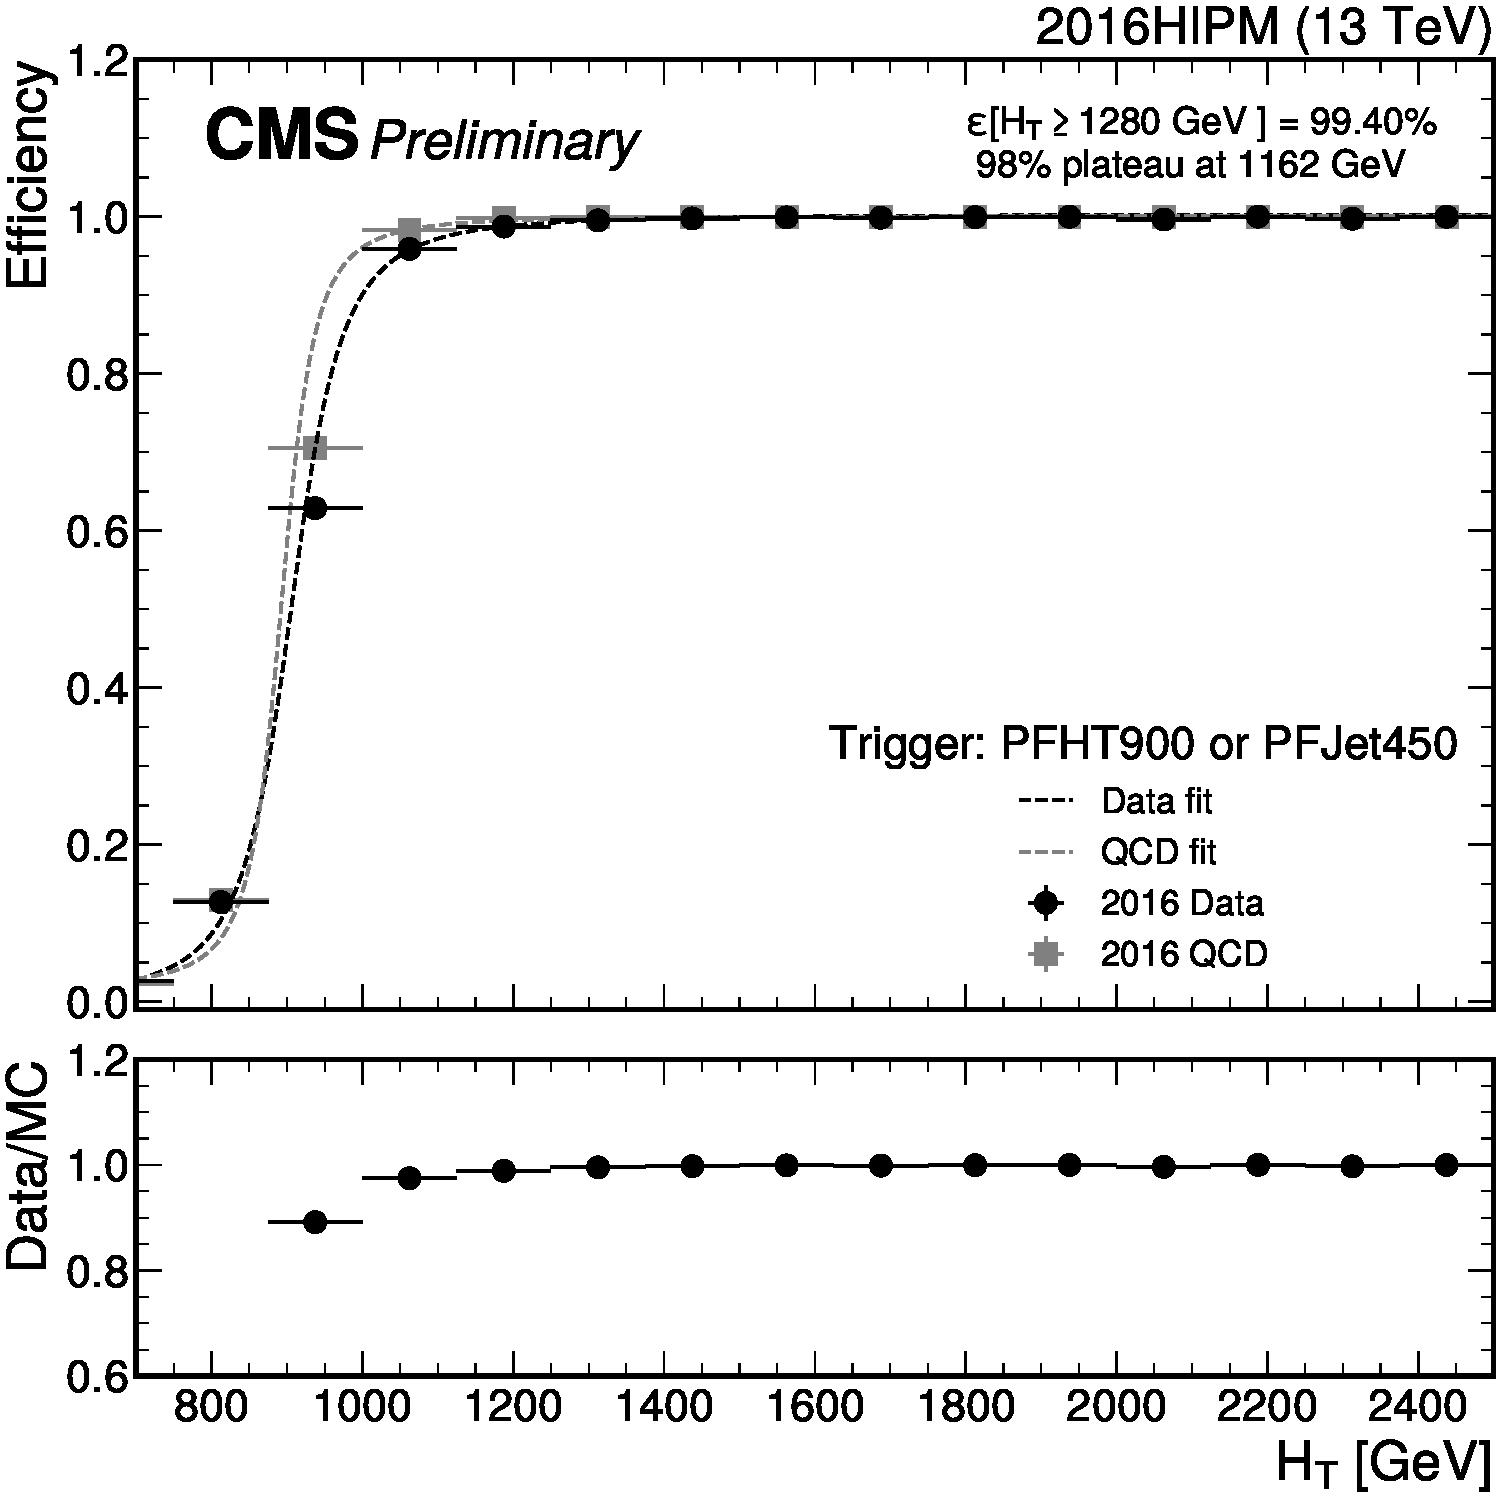
\includegraphics[width=\linewidth]{Images/pdfs/16-APV-HIPM_efficiency_withratio_and_fits.pdf}
		\caption{Run2 2016 HIPM}
		\label{fig:HT_eff_16_HIPM}
	\end{subfigure}

	\begin{subfigure}{.45\textwidth}
		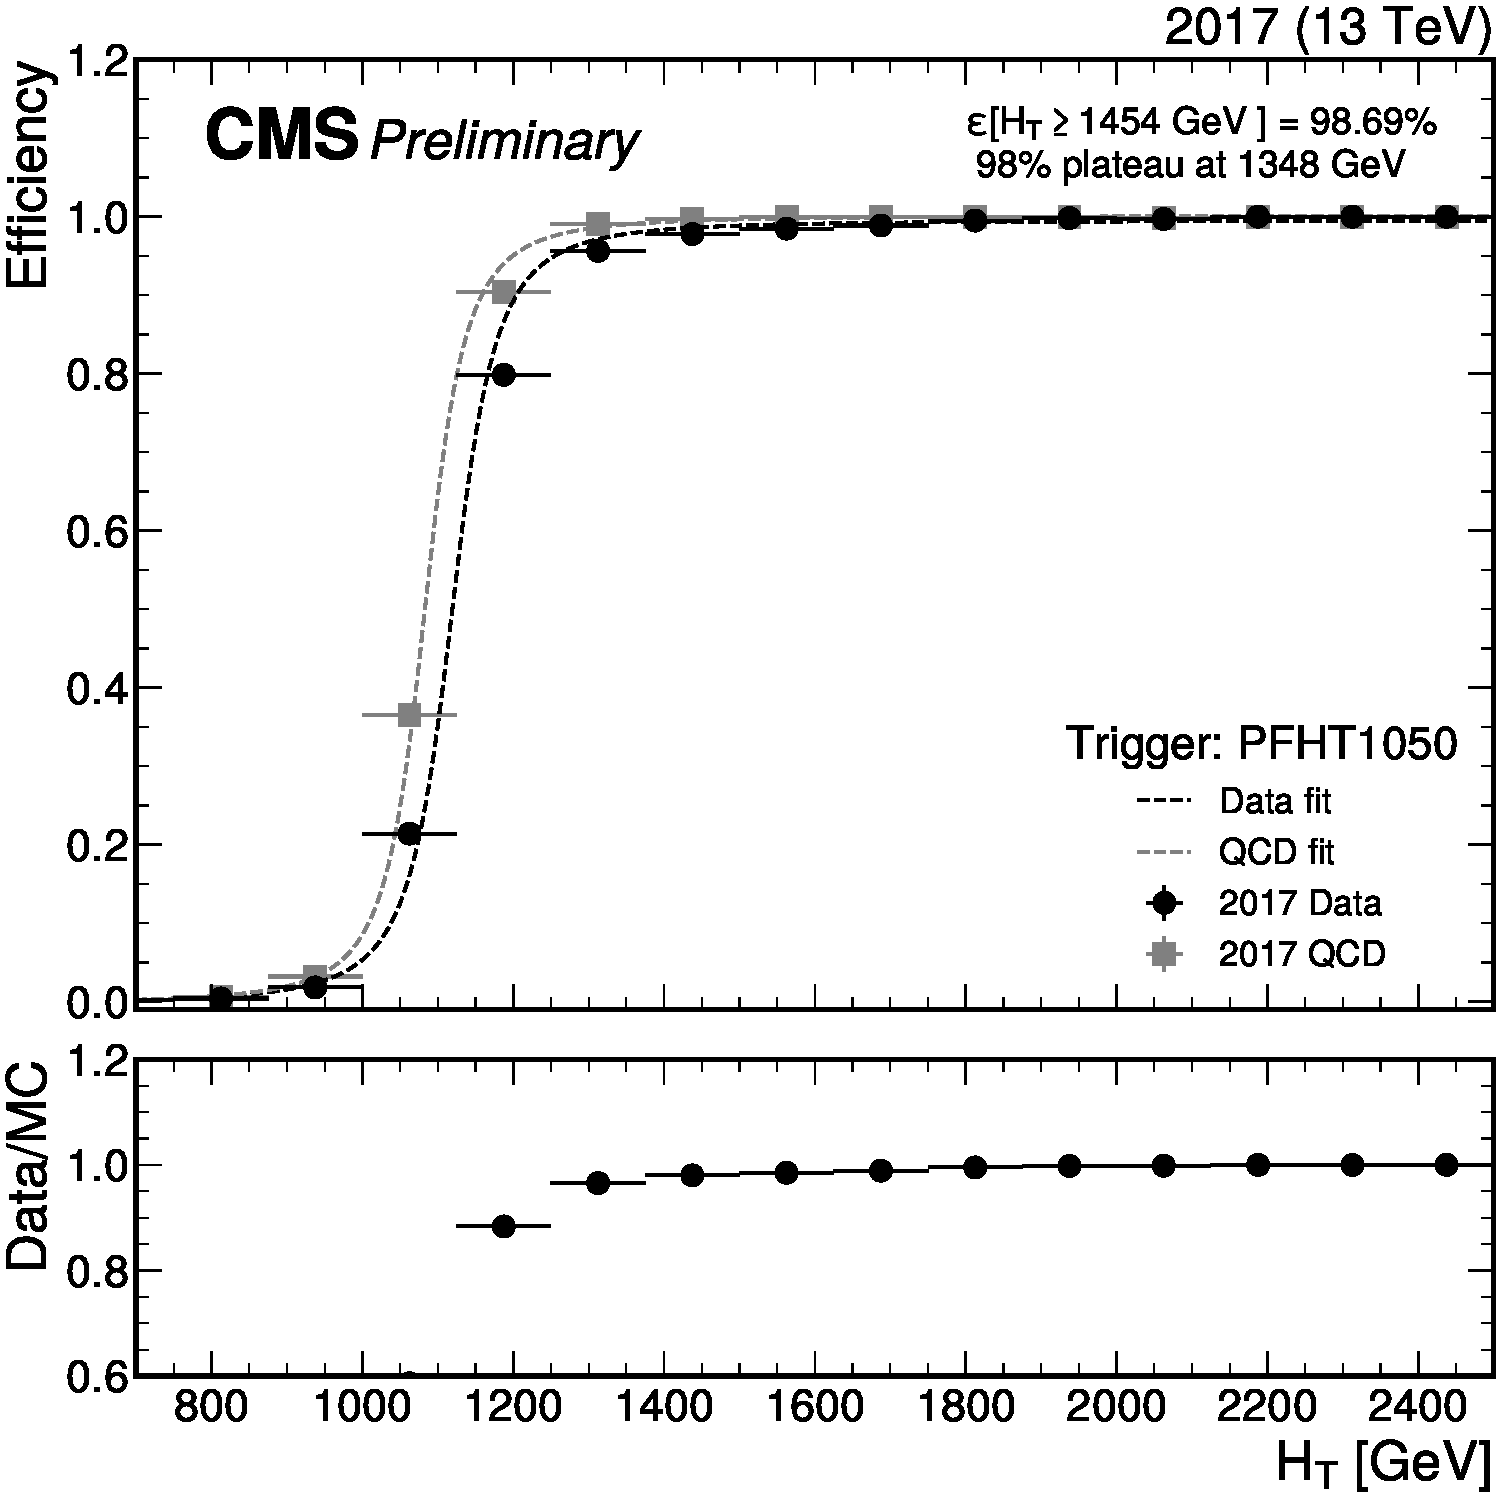
\includegraphics[width=\linewidth]{Images/pdfs/17_efficiency_withratio_and_fits.pdf}
		\caption{Run2 2017}
		\label{fig:HT_eff_17}
	\end{subfigure}
	%
	\begin{subfigure}{.45\textwidth}
		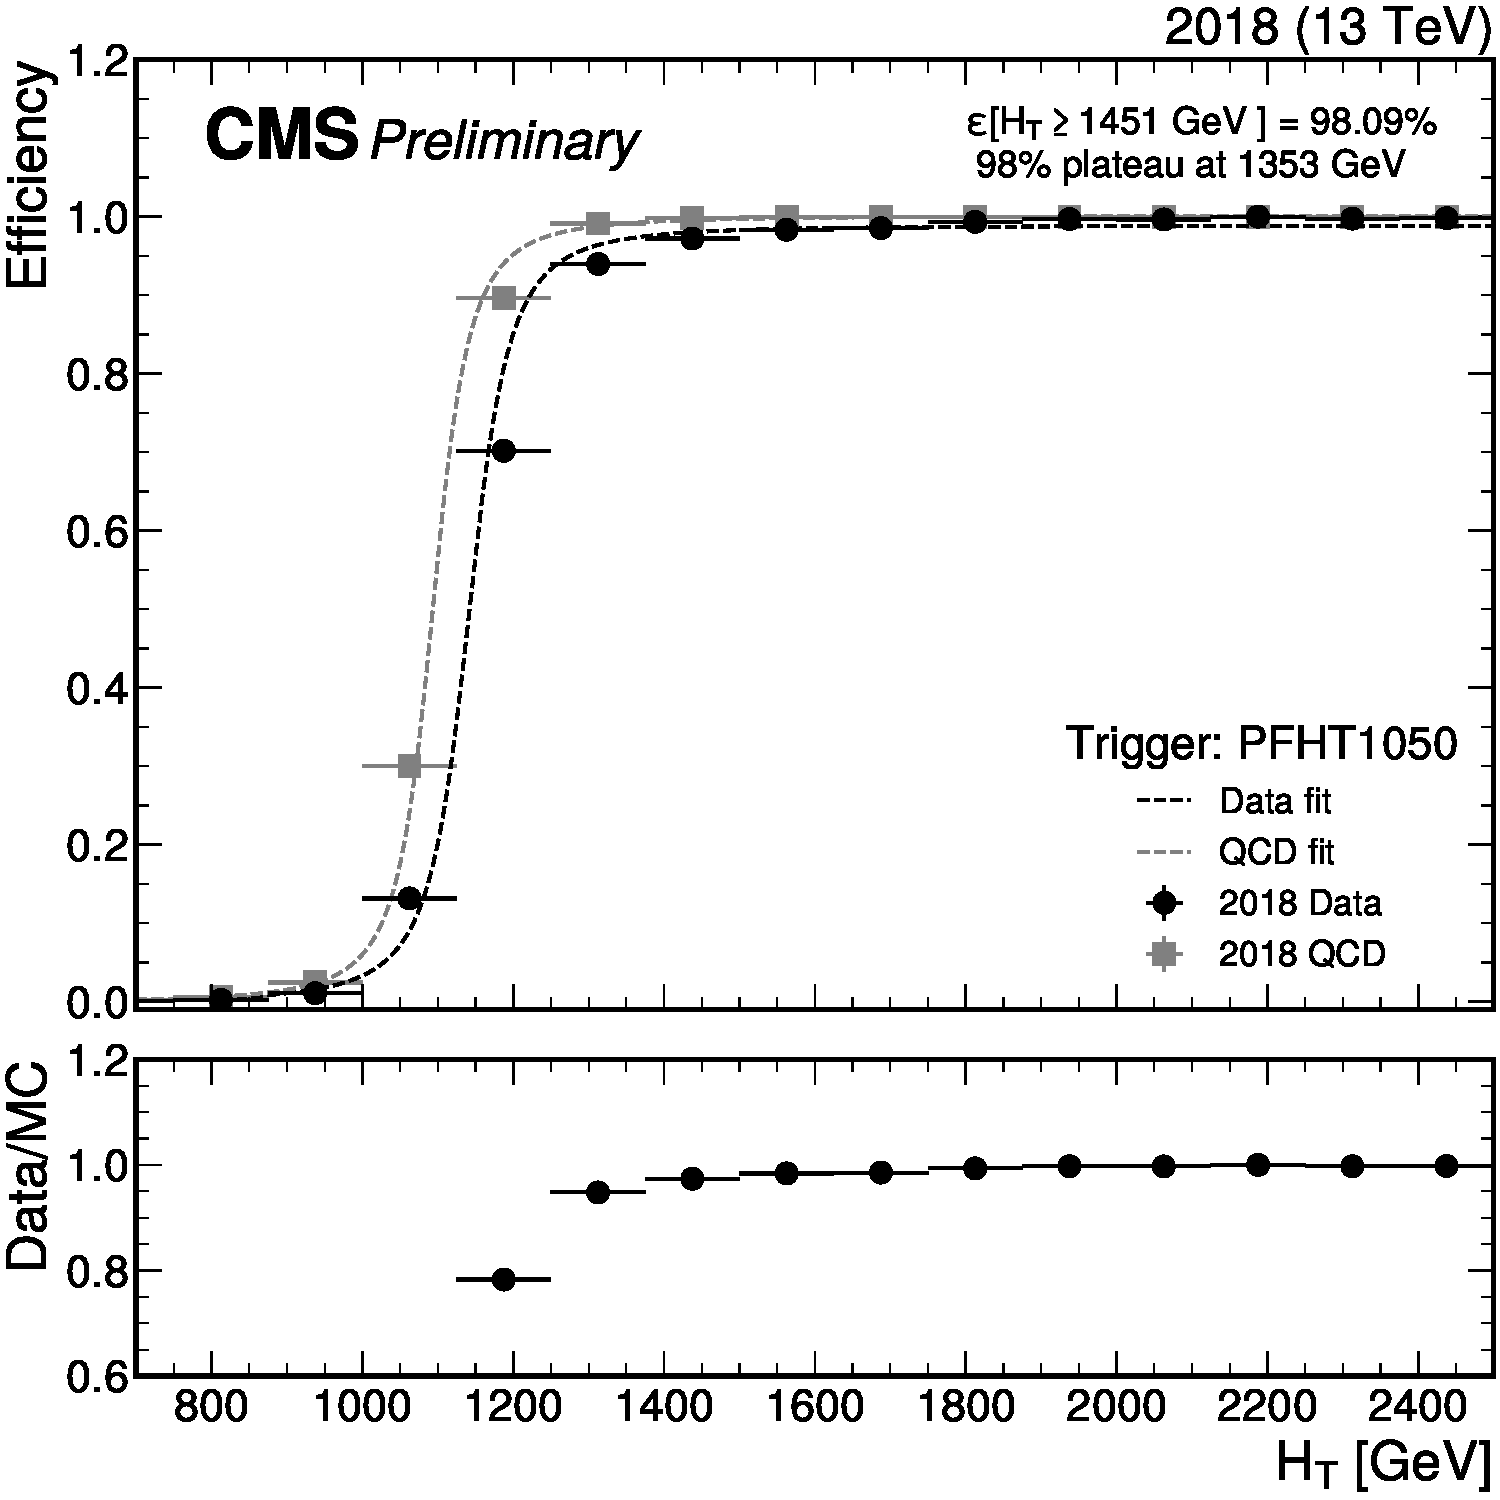
\includegraphics[width=\linewidth]{Images/pdfs/18_efficiency_withratio_and_fits.pdf}
		\caption{Run2 2018}
		\label{fig:HT_eff_18}
	\end{subfigure}
	\caption[Comparison of trigger efficiencies for \HT trigger]{Comparison of efficiency for \HT trigger as a function of event \HT measured relative to \texttt{HLT\_Mu50\_v*} in data (black) and QCD MC (gray) and fit to the algebraic function \textit{f} (line).}
	\label{fig:HT_efficiencies}
\end{figure}

The scale factor values used for signal MC can be found in \Cref{tab:2016_triggerSF,tab:2016HIPM_triggerSF,tab:2017_triggerSF,tab:2018_triggerSF}. The uncertainties in the table are just the statistical uncertainties of data and MC selection efficiency propagated appropriately.


\begin{table}
	\centering
	\caption{Scale factors (SF) and statistical uncertainties of the \HT trigger for 2016.}
	\label{tab:2016_triggerSF}
	\begin{tabular}{cccc}
		\hline
		\HT bin[GeV]    & SF       & uncertainty (upper) & uncertainty (lower) \\
		\hline
		1200.0 - 1375.0 & 0.987578 & 0.001114            & 0.001227            \\
		1375.0 - 1500.0 & 0.993525 & 0.001043            & 0.001235            \\
		1500.0 - 1625.0 & 0.998121 & 0.000693            & 0.001015            \\
		1625.0 - 1750.0 & 0.998326 & 0.000801            & 0.001325            \\
		1750.0 - 1875.0 & 1.001928 & 0.000708            & 0.001671            \\
		1875.0 - 2000.0 & 0.998974 & 0.000848            & 0.002358            \\
		2000.0 - 2125.0 & 1.006414 & 0.000855            & 0.002898            \\
		2125.0 - 2250.0 & 0.997732 & 0.001876            & 0.005197            \\
		2250.0 - 2375.0 & 1.000000 & 0.000000            & 0.006580            \\
		2375.0 - 2500.0 & 1.000000 & 0.000000            & 0.009449            \\
		\hline
	\end{tabular}
\end{table}

\begin{table}
	\centering
	\caption{Scale factors (SF) and statistical uncertainties of the \HT trigger for 2016HIPM.}
	\label{tab:2016HIPM_triggerSF}
	\begin{tabular}{cccc}
		\hline
		\HT bin[GeV]    & SF       & uncertainty (upper) & uncertainty (lower) \\
		\hline
		1200.0 - 1375.0 & 0.995561 & 0.000618            & 0.000723            \\
		1375.0 - 1500.0 & 0.997767 & 0.000536            & 0.000697            \\
		1500.0 - 1625.0 & 0.999147 & 0.000408            & 0.000682            \\
		1625.0 - 1750.0 & 0.998692 & 0.000626            & 0.001037            \\
		1750.0 - 1875.0 & 0.999505 & 0.000410            & 0.001143            \\
		1875.0 - 2000.0 & 1.000000 & 0.000000            & 0.001484            \\
		2000.0 - 2125.0 & 0.996381 & 0.001969            & 0.003510            \\
		2125.0 - 2250.0 & 1.000000 & 0.000000            & 0.003497            \\
		2250.0 - 2375.0 & 0.997389 & 0.002160            & 0.005981            \\
		2375.0 - 2500.0 & 1.000000 & 0.000000            & 0.006582            \\
		\hline
	\end{tabular}
\end{table}

\begin{table}
	\centering
	\caption{Scale factors and statistical uncertainties of the \HT trigger for 2017.}
	\label{tab:2017_triggerSF}
	\begin{tabular}{cccc}
		\hline
		\HT bin[GeV]    & SF       & uncertainty (upper) & uncertainty (lower) \\
		\hline
		1200.0 - 1375.0 & 0.965681 & 0.001357            & 0.001412            \\
		1375.0 - 1500.0 & 0.980217 & 0.001125            & 0.001199            \\
		1500.0 - 1625.0 & 0.985178 & 0.001111            & 0.001201            \\
		1625.0 - 1750.0 & 0.989094 & 0.001191            & 0.001328            \\
		1750.0 - 1875.0 & 0.995385 & 0.000992            & 0.001215            \\
		1875.0 - 2000.0 & 0.998218 & 0.000735            & 0.001111            \\
		2000.0 - 2125.0 & 0.998595 & 0.001134            & 0.001635            \\
		2125.0 - 2250.0 & 1.000000 & 0.000000            & 0.001187            \\
		2250.0 - 2375.0 & 1.000000 & 0.000000            & 0.001821            \\
		2375.0 - 2500.0 & 1.000277 & 0.000166            & 0.002397            \\
		2500.0 - 2625.0 & 1.005464 & 0.001036            & 0.003895            \\
		\hline
	\end{tabular}
\end{table}

\begin{table}
	\centering
	\caption{Scale factors and statistical uncertainties of the \HT trigger for 2018.}
	\label{tab:2018_triggerSF}
	\begin{tabular}{cccc}
		\hline
		\HT bin[GeV]    & SF       & uncertainty (upper) & uncertainty (lower) \\
		\hline
		1200.0 - 1375.0 & 0.947967 & 0.001657            & 0.001723            \\
		1375.0 - 1500.0 & 0.973940 & 0.001332            & 0.001409            \\
		1500.0 - 1625.0 & 0.983915 & 0.001286            & 0.001392            \\
		1625.0 - 1750.0 & 0.985506 & 0.001518            & 0.001685            \\
		1750.0 - 1875.0 & 0.993555 & 0.001249            & 0.001515            \\
		1875.0 - 2000.0 & 0.997541 & 0.001054            & 0.001498            \\
		2000.0 - 2125.0 & 0.997264 & 0.001403            & 0.002103            \\
		2125.0 - 2250.0 & 1.000000 & 0.000000            & 0.001596            \\
		2250.0 - 2375.0 & 0.997558 & 0.001577            & 0.003217            \\
		2375.0 - 2500.0 & 0.998141 & 0.001538            & 0.004268            \\
		\hline
	\end{tabular}
\end{table}

For completeness we also checked the trigger efficiencies in a region of phase-space were we expect to be signal-free (i.e. SinglePhoton data stream). We see in a similar fashion the plots for these unprescaled triggers divided by year in \Cref{fig:HT_eff_SinglePhoton_16,fig:HT_eff_SinglePhoton_16_HIPM,fig:HT_eff_SinglePhoton_17,fig:HT_eff_SinglePhoton_18}.
More detailed plots of the fit functions around the turn-on region can be found in \Cref{fig:fits}
that show the $H_T$ trigger efficiencies in each fit.



\begin{figure}
	\centering
	\begin{subfigure}{.45\textwidth}
		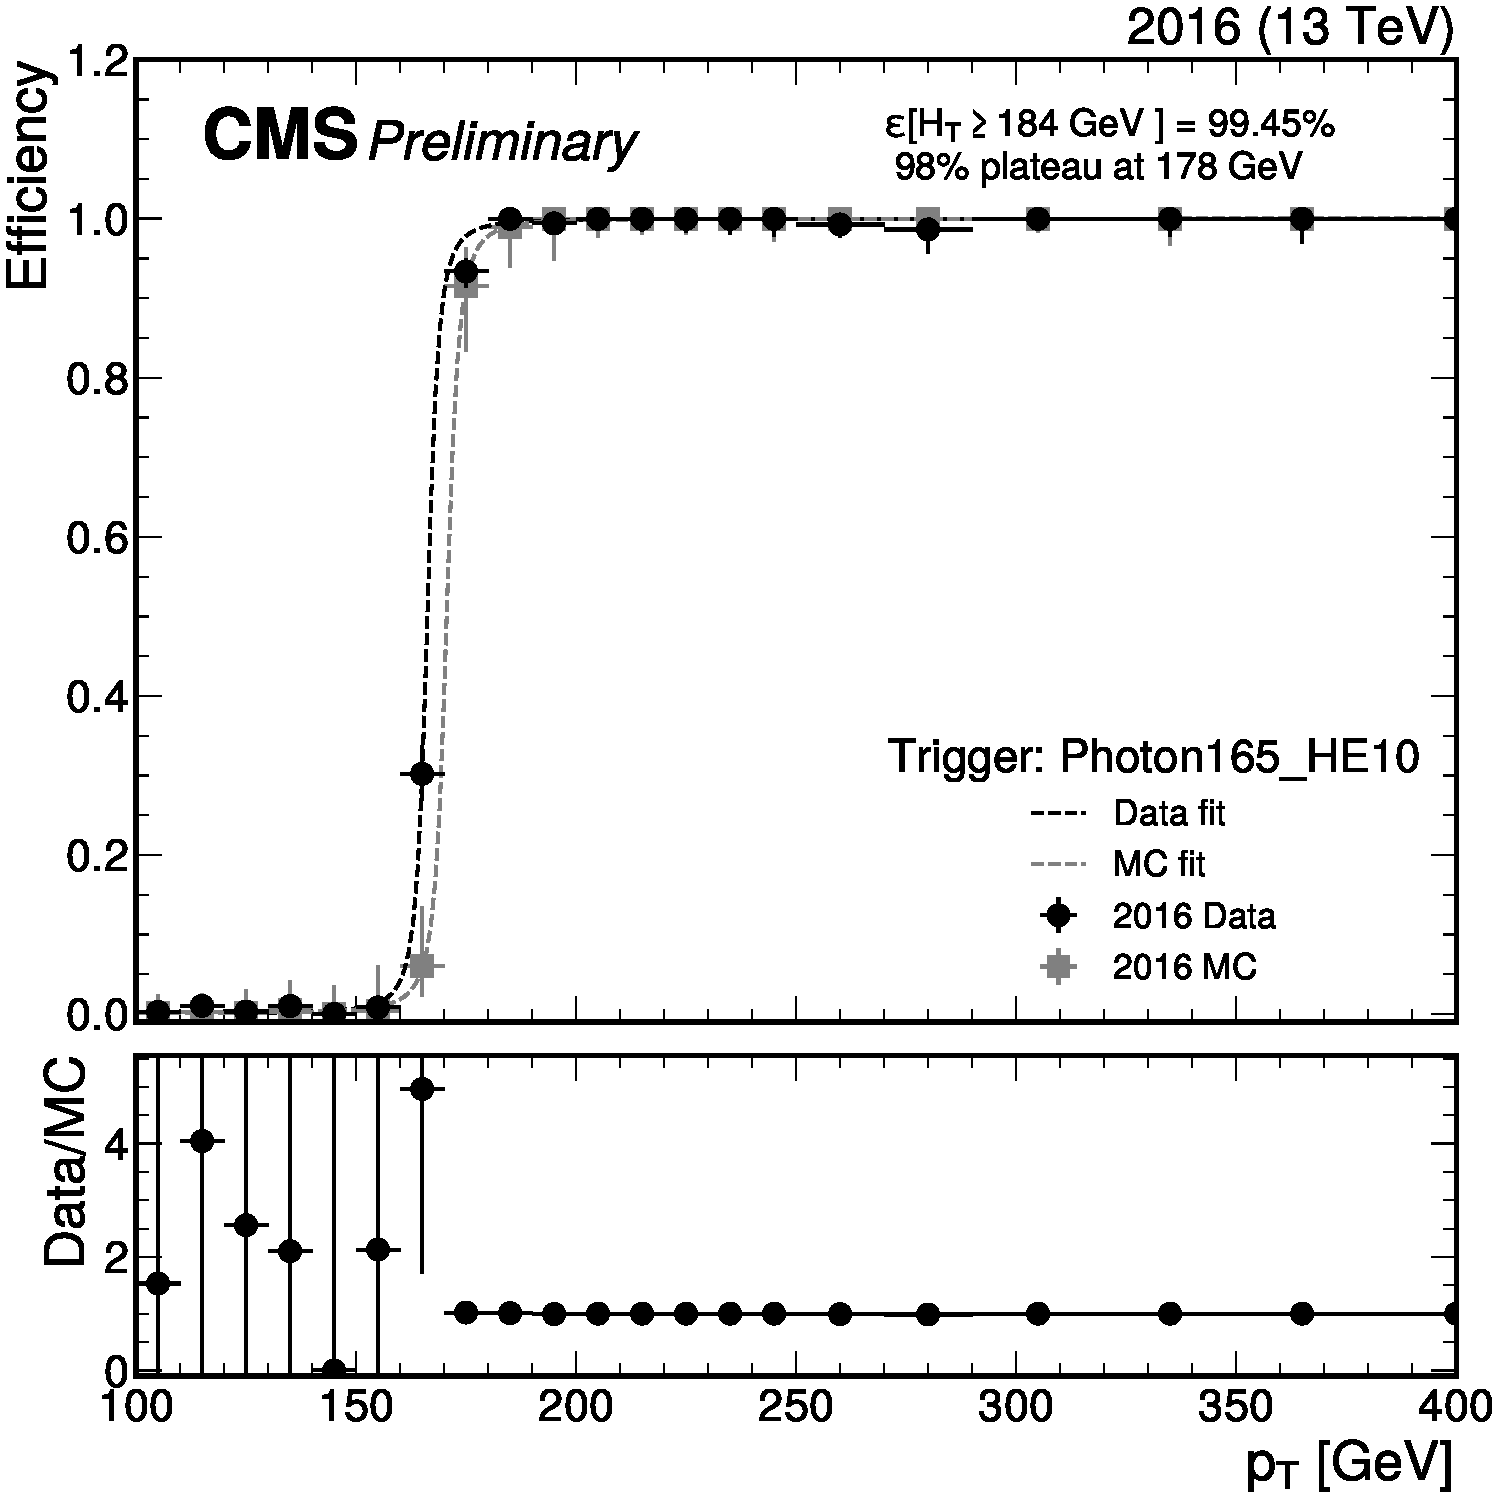
\includegraphics[width=\linewidth]{Images/pdfs/16_SinglePhoton_efficiency_withratio_and_fits.pdf}
		\caption{Run2 SinglePhoton 2016}
		\label{fig:HT_eff_SinglePhoton_16}
	\end{subfigure}
	%
	\begin{subfigure}{.45\textwidth}
		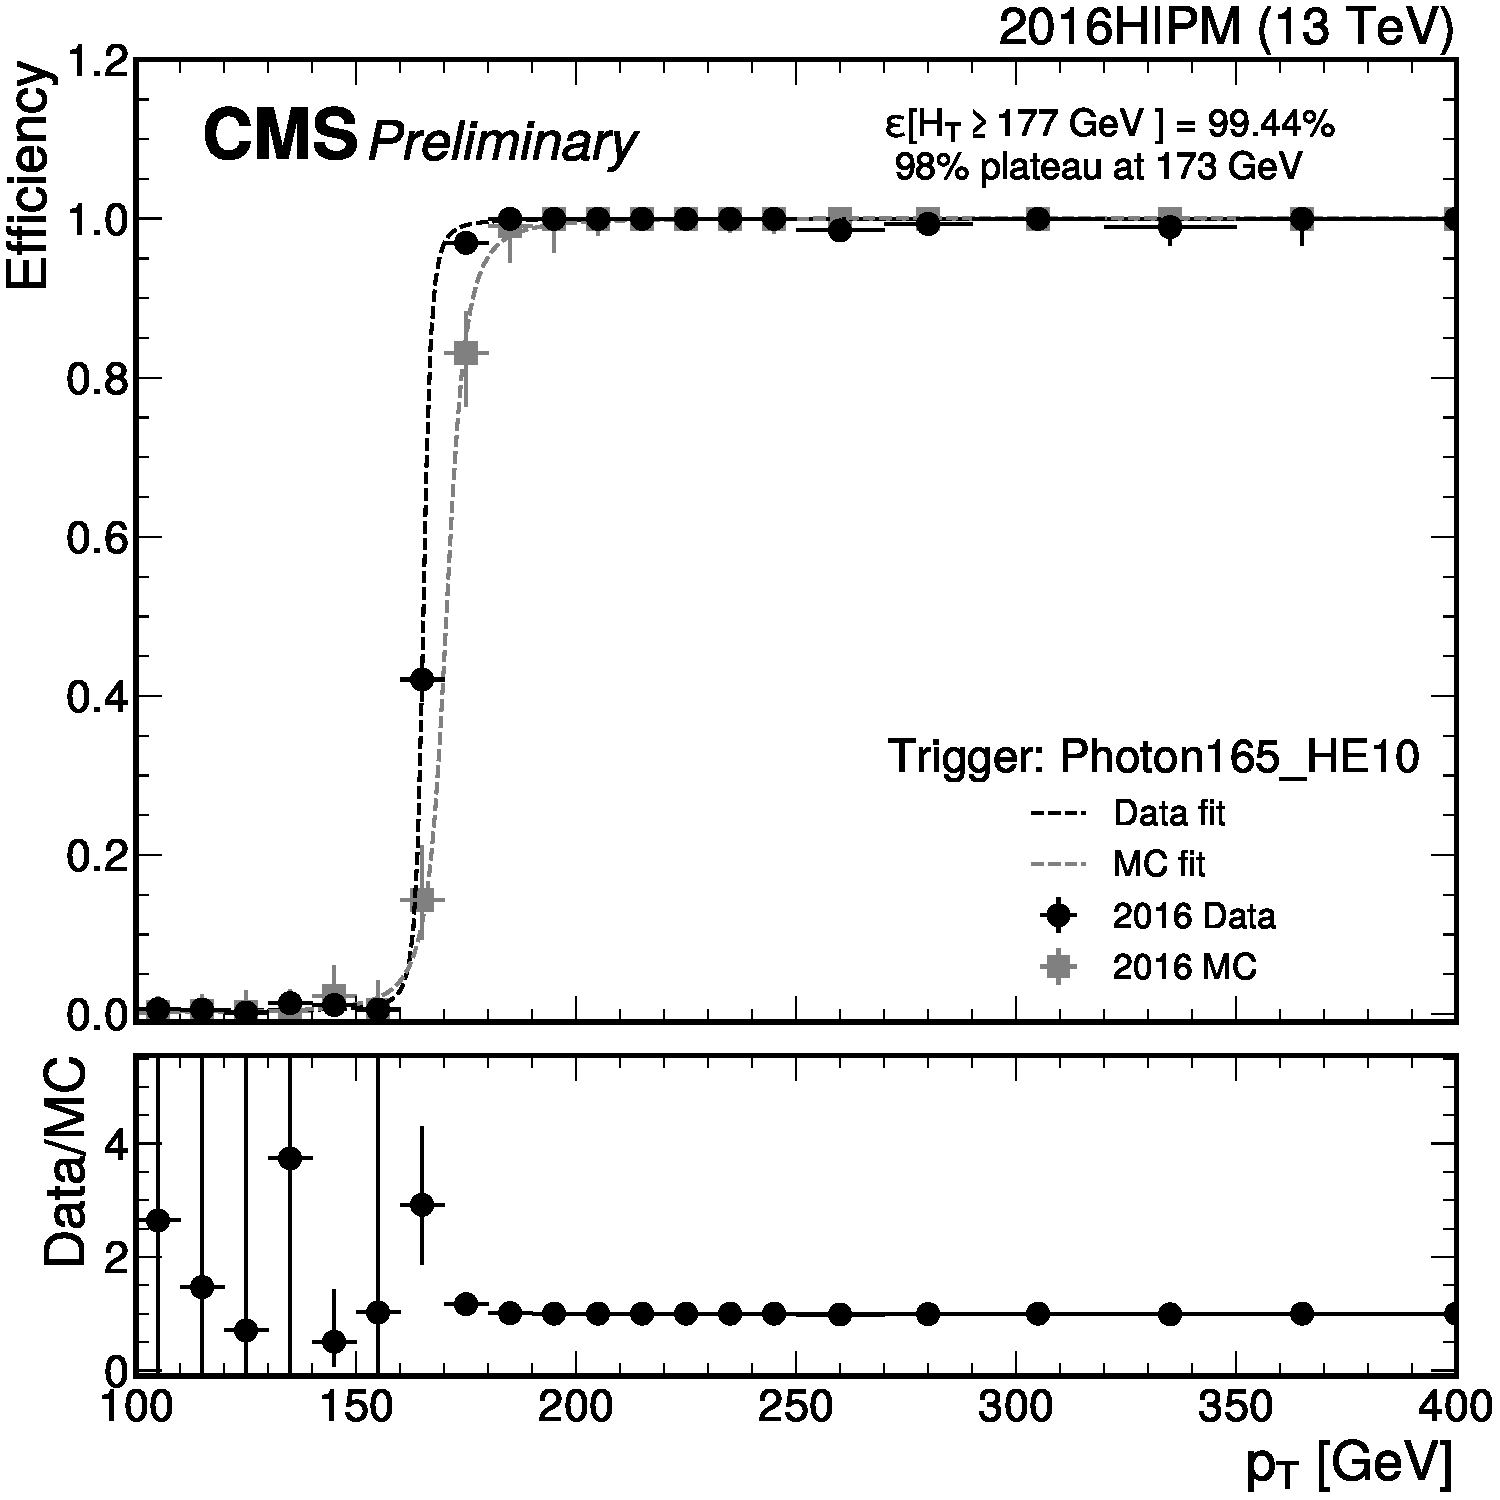
\includegraphics[width=\linewidth]{Images/pdfs/16-APV-HIPM_SinglePhoton_efficiency_withratio_and_fits.pdf}
		\caption{Run2 SinglePhoton 2016 HIPM}
		\label{fig:HT_eff_SinglePhoton_16_HIPM}
	\end{subfigure}

	\begin{subfigure}{.45\textwidth}
		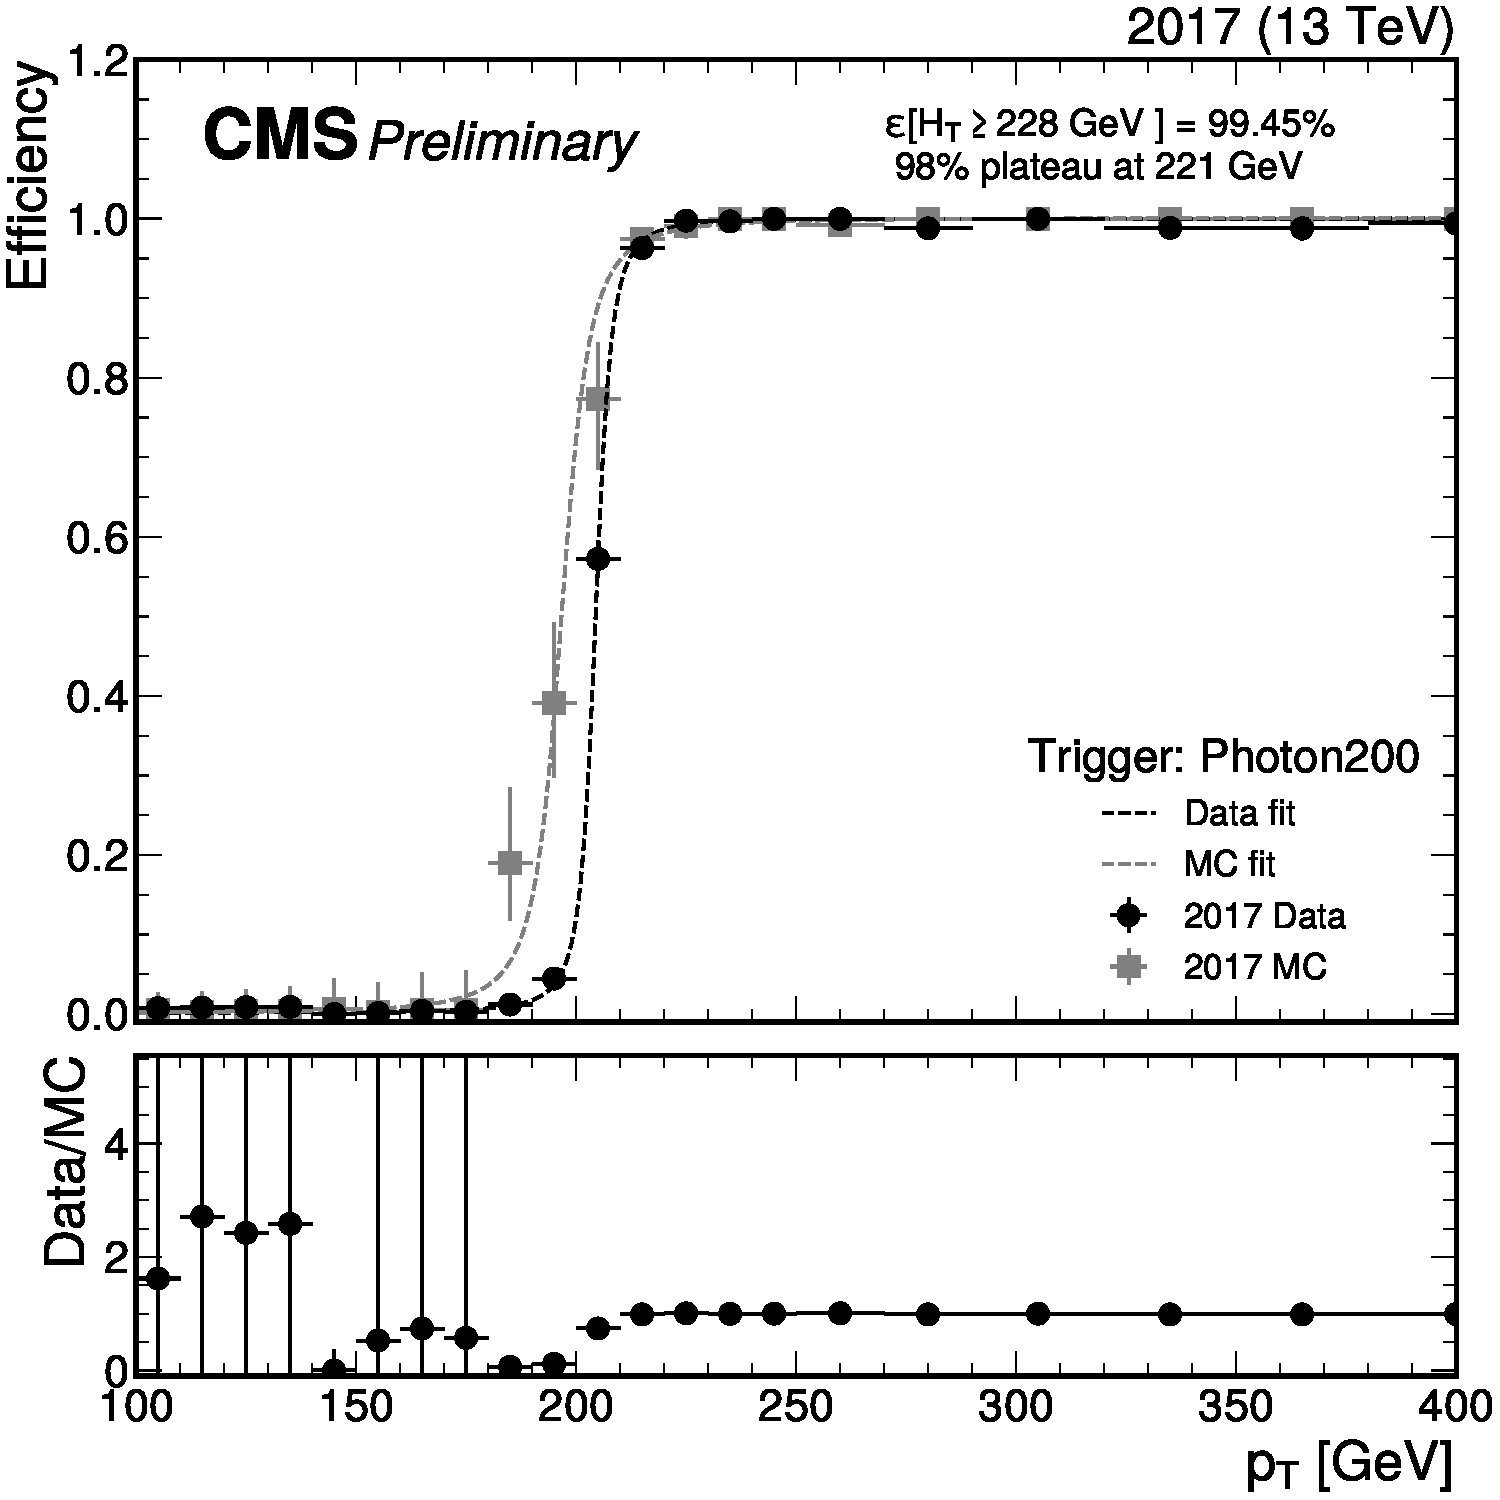
\includegraphics[width=\linewidth]{Images/pdfs/17_SinglePhoton_efficiency_withratio_and_fits.pdf}
		\caption{Run2 SinglePhoton 2017}
		\label{fig:HT_eff_SinglePhoton_17}
	\end{subfigure}
	%
	\begin{subfigure}{.45\textwidth}
		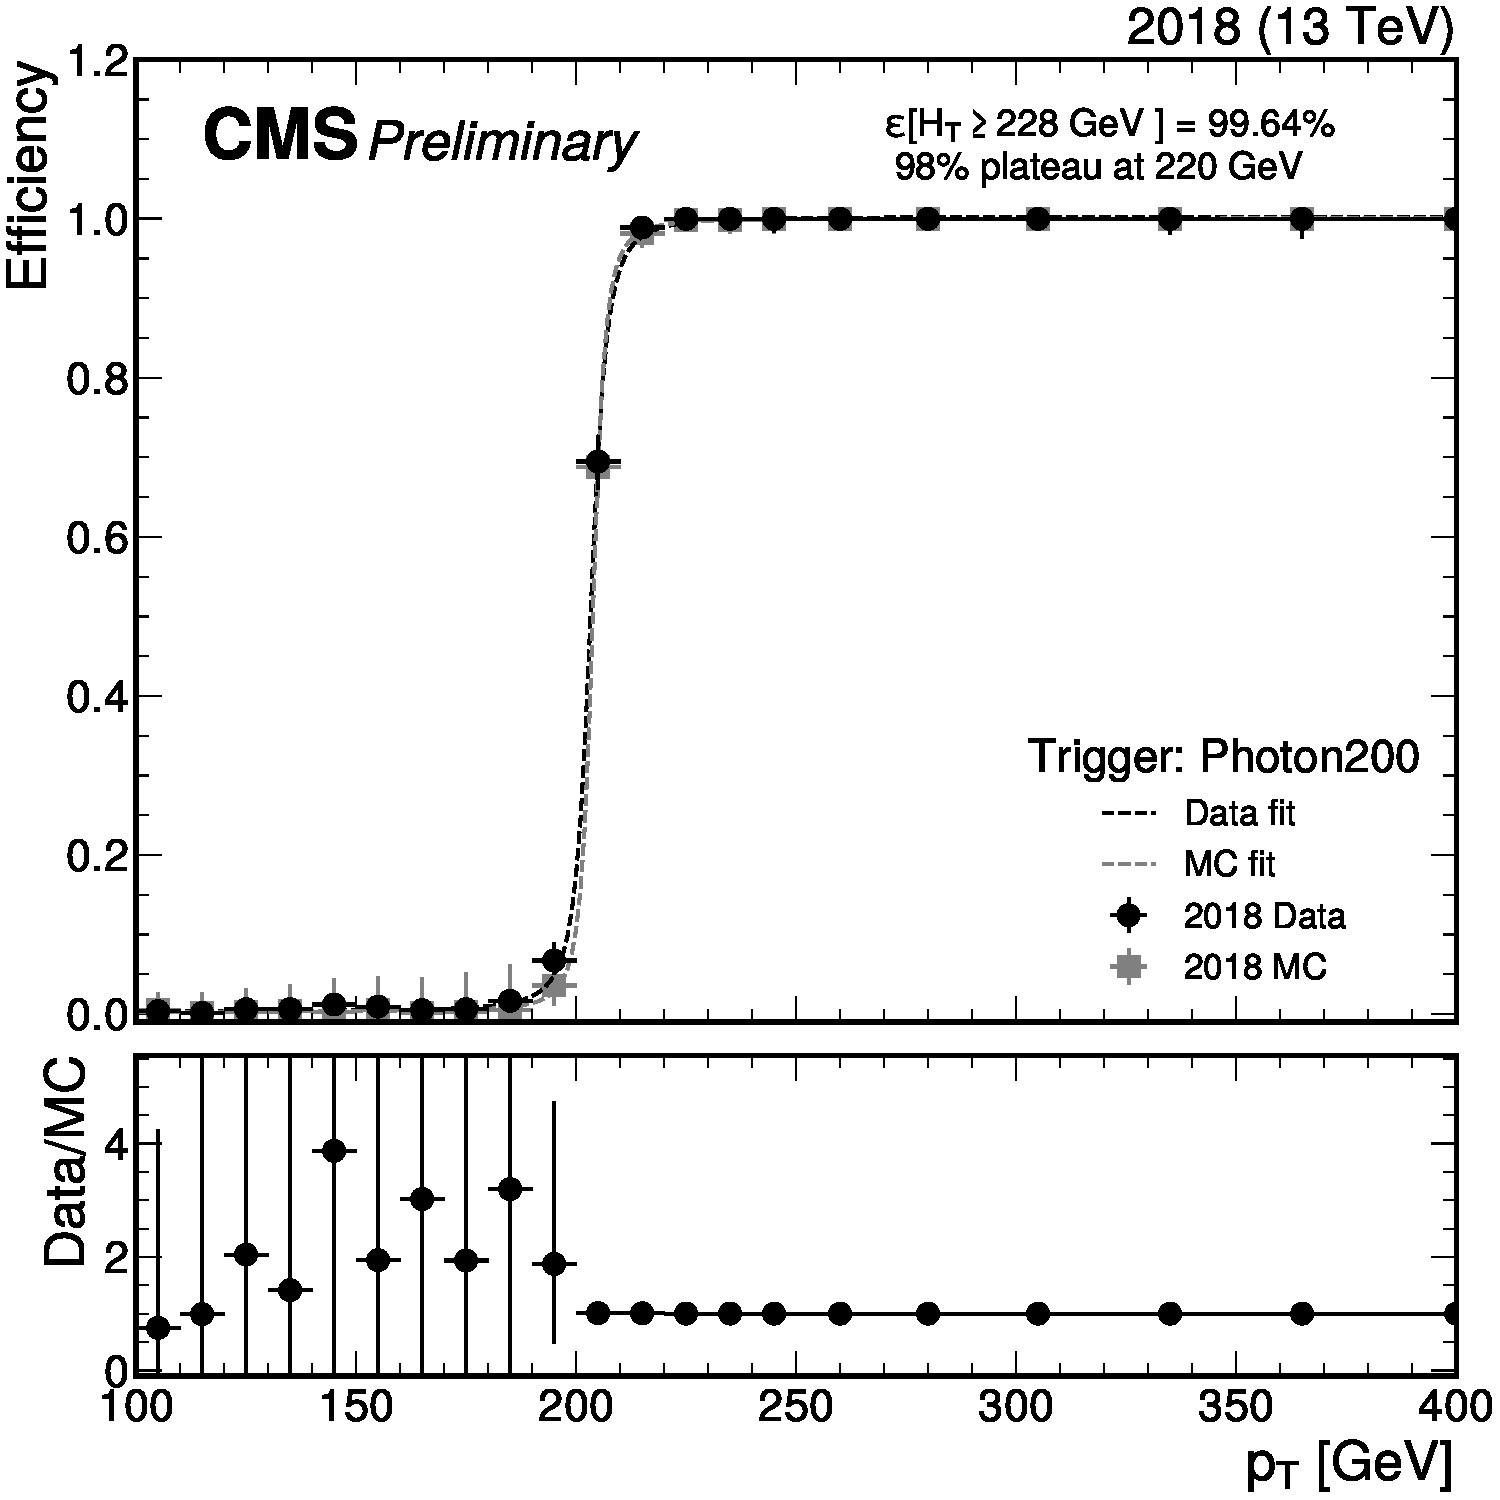
\includegraphics[width=\linewidth]{Images/pdfs/18_SinglePhoton_efficiency_withratio_and_fits.pdf}
		\caption{Run2 SinglePhoton 2018}
		\label{fig:HT_eff_SinglePhoton_18}
	\end{subfigure}
	\caption[Comparison of trigger efficiencies for \HT trigger for the signal free region.]{Comparison of efficiency for $p_T$ trigger as a function of  jet $p_T$ for the SinglePhoton data stream. Measured relative to \texttt{HLT\_Mu50\_v*} in data (black) and QCD MC (gray) and fit to the algebraic function \textit{f} (line).}
\end{figure}


\begin{figure}
	\centering
	\begin{subfigure}{.36\linewidth}
		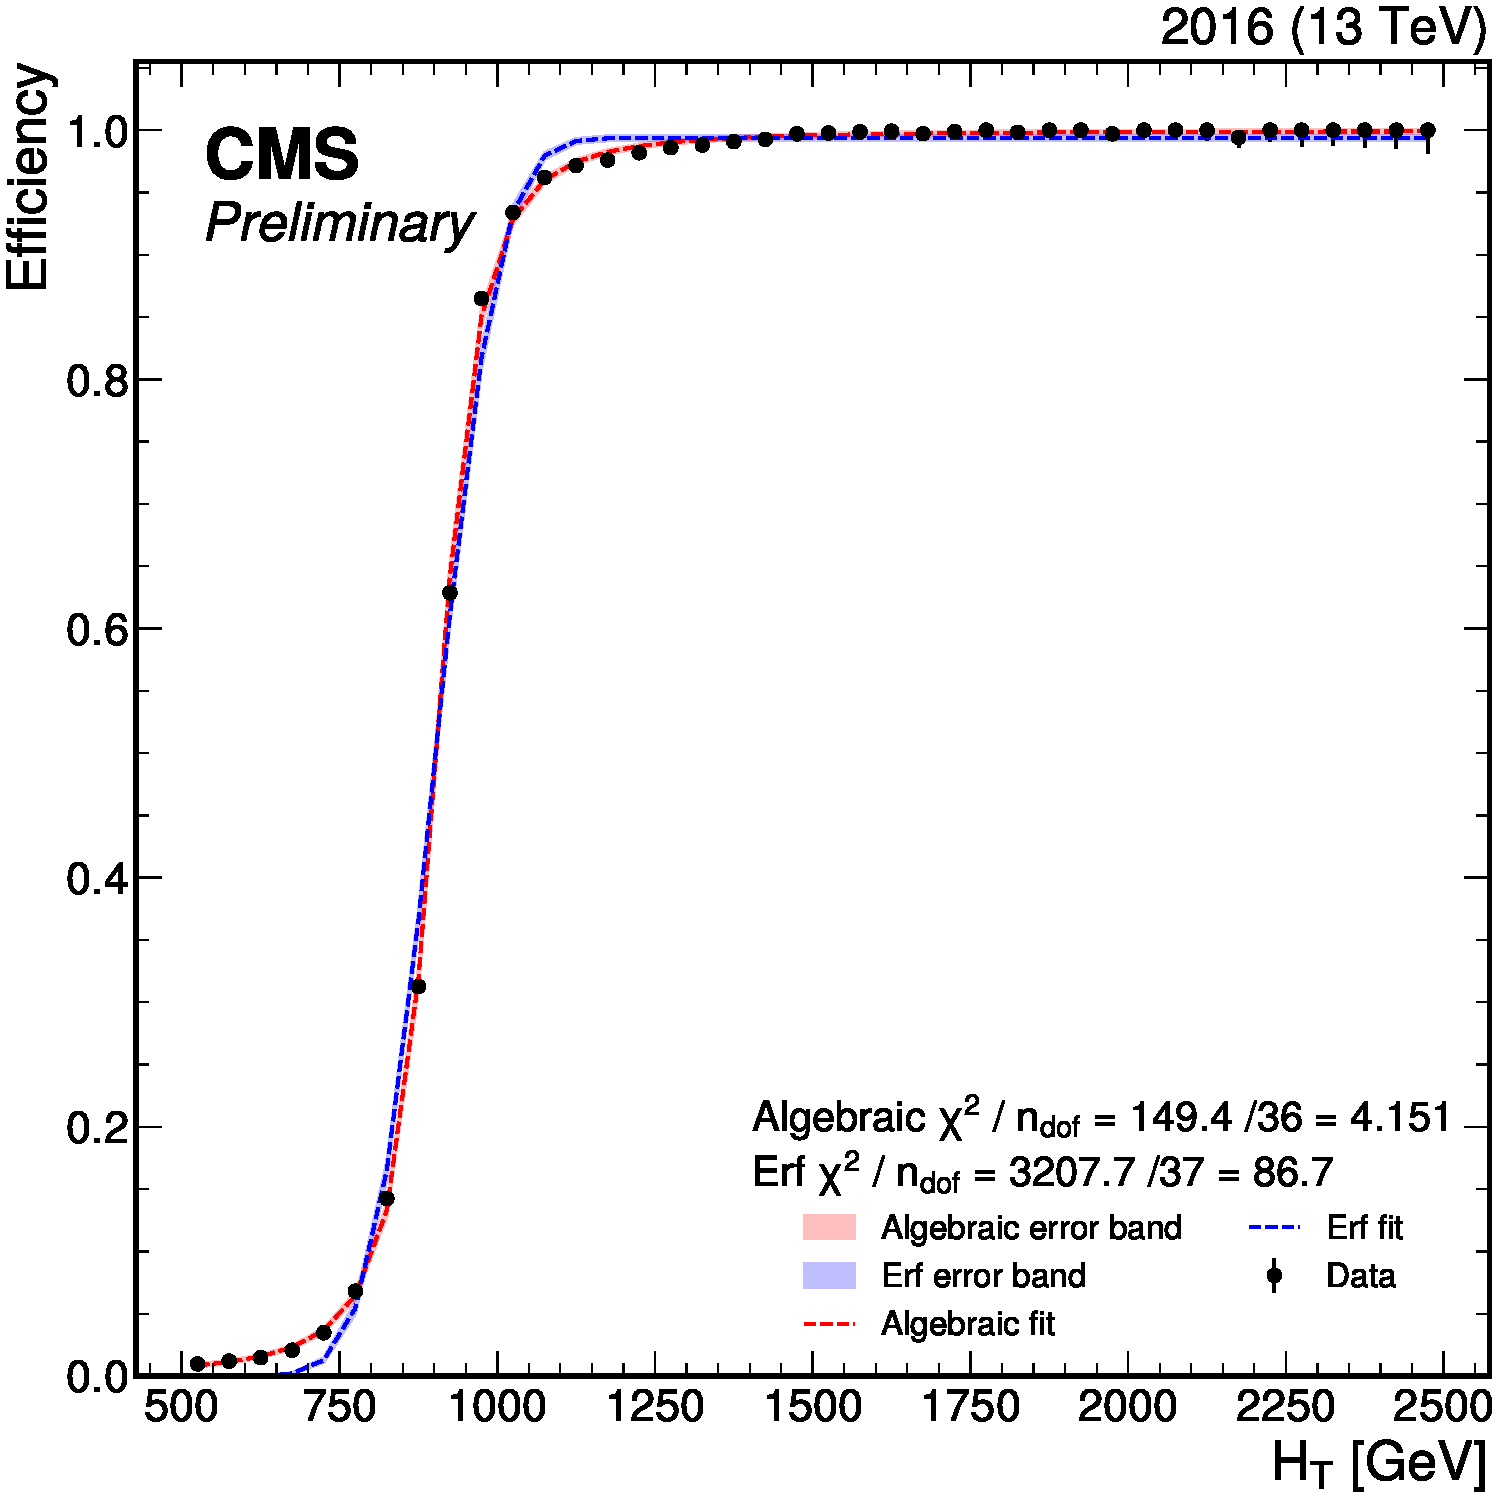
\includegraphics[width=\linewidth]{Images/pdfs/fits_16.pdf}
		% \caption{Caption}
		% \label{fig:enter-label}
	\end{subfigure}%
	\begin{subfigure}{.36\linewidth}
		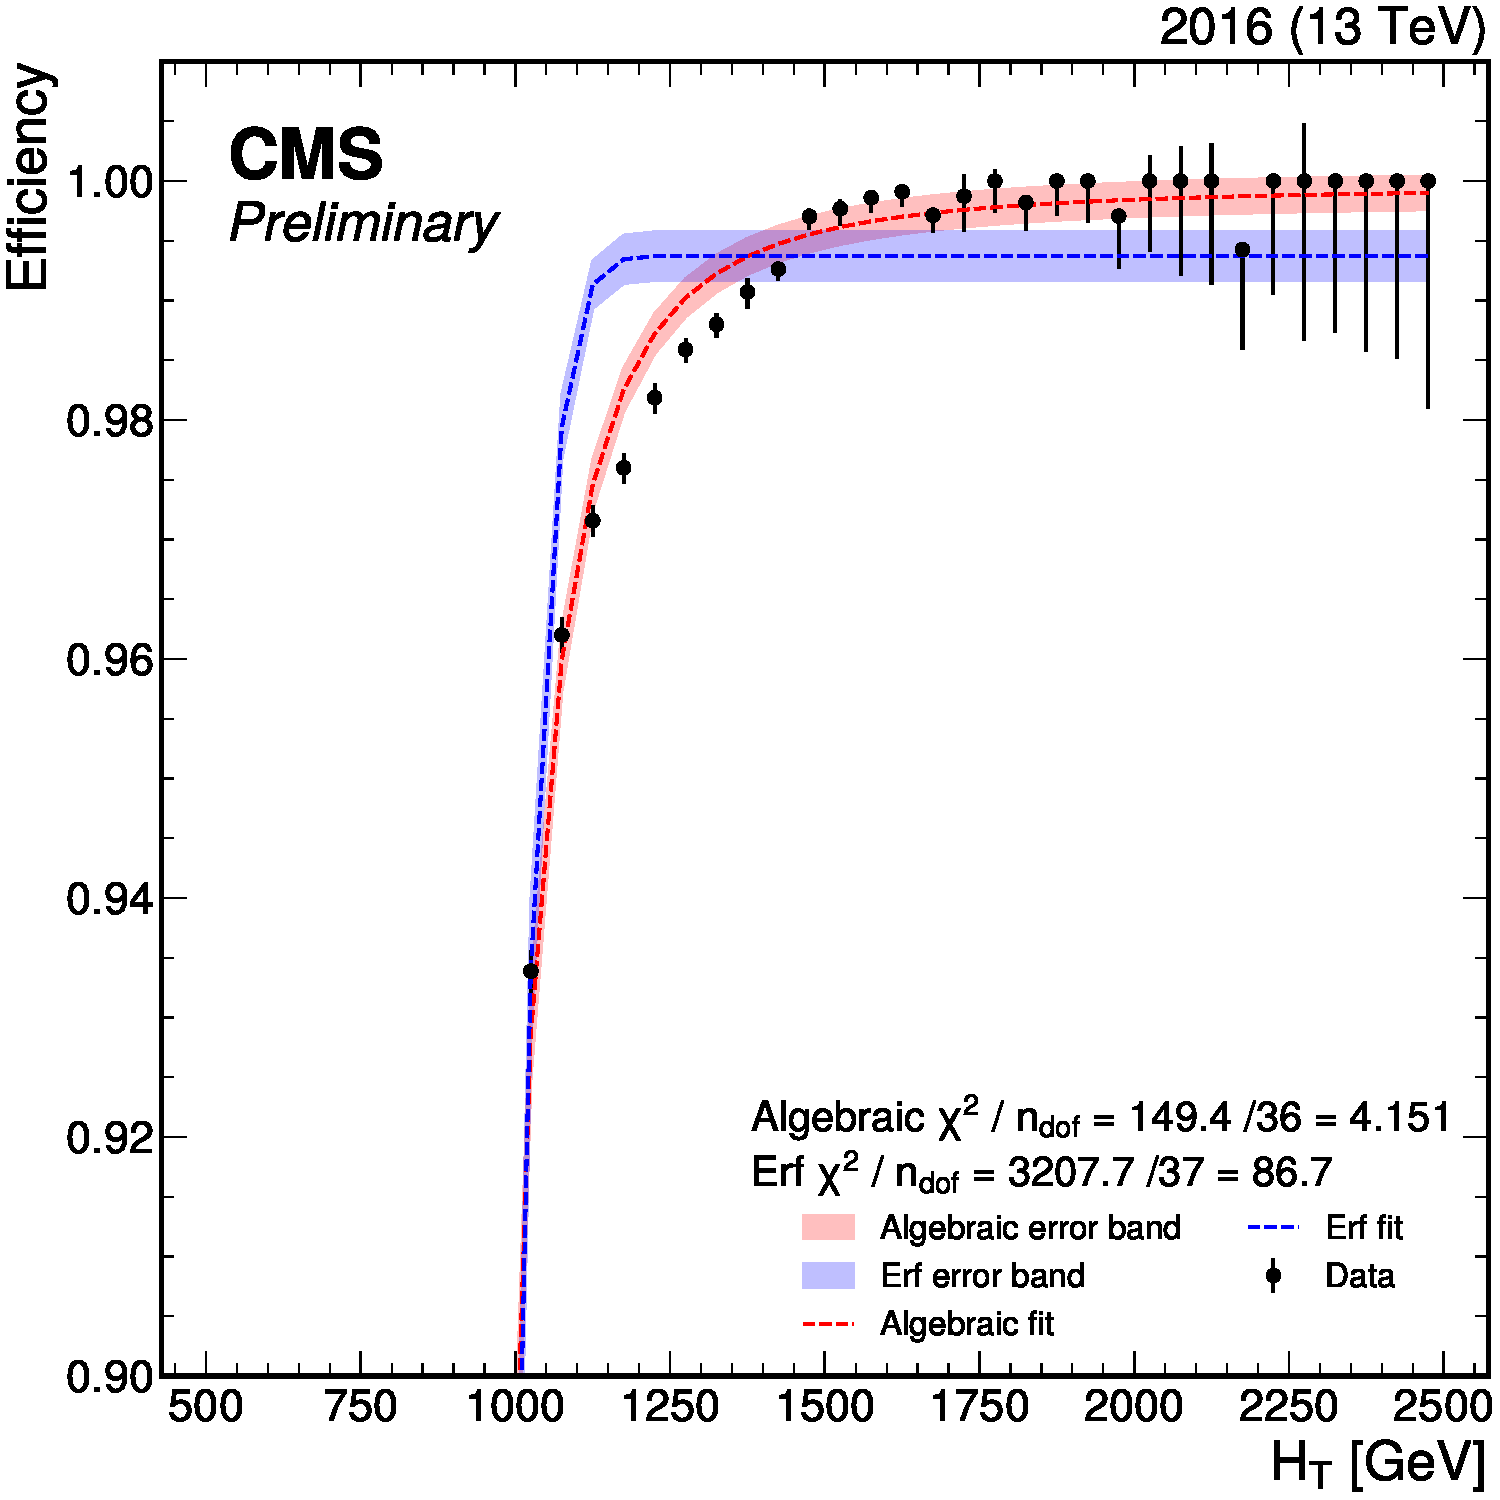
\includegraphics[width=\linewidth]{Images/pdfs/fits_closeup_16.pdf}
		% \caption{Caption}
		% \label{fig:enter-label}
	\end{subfigure}
	\begin{subfigure}{.36\linewidth}
		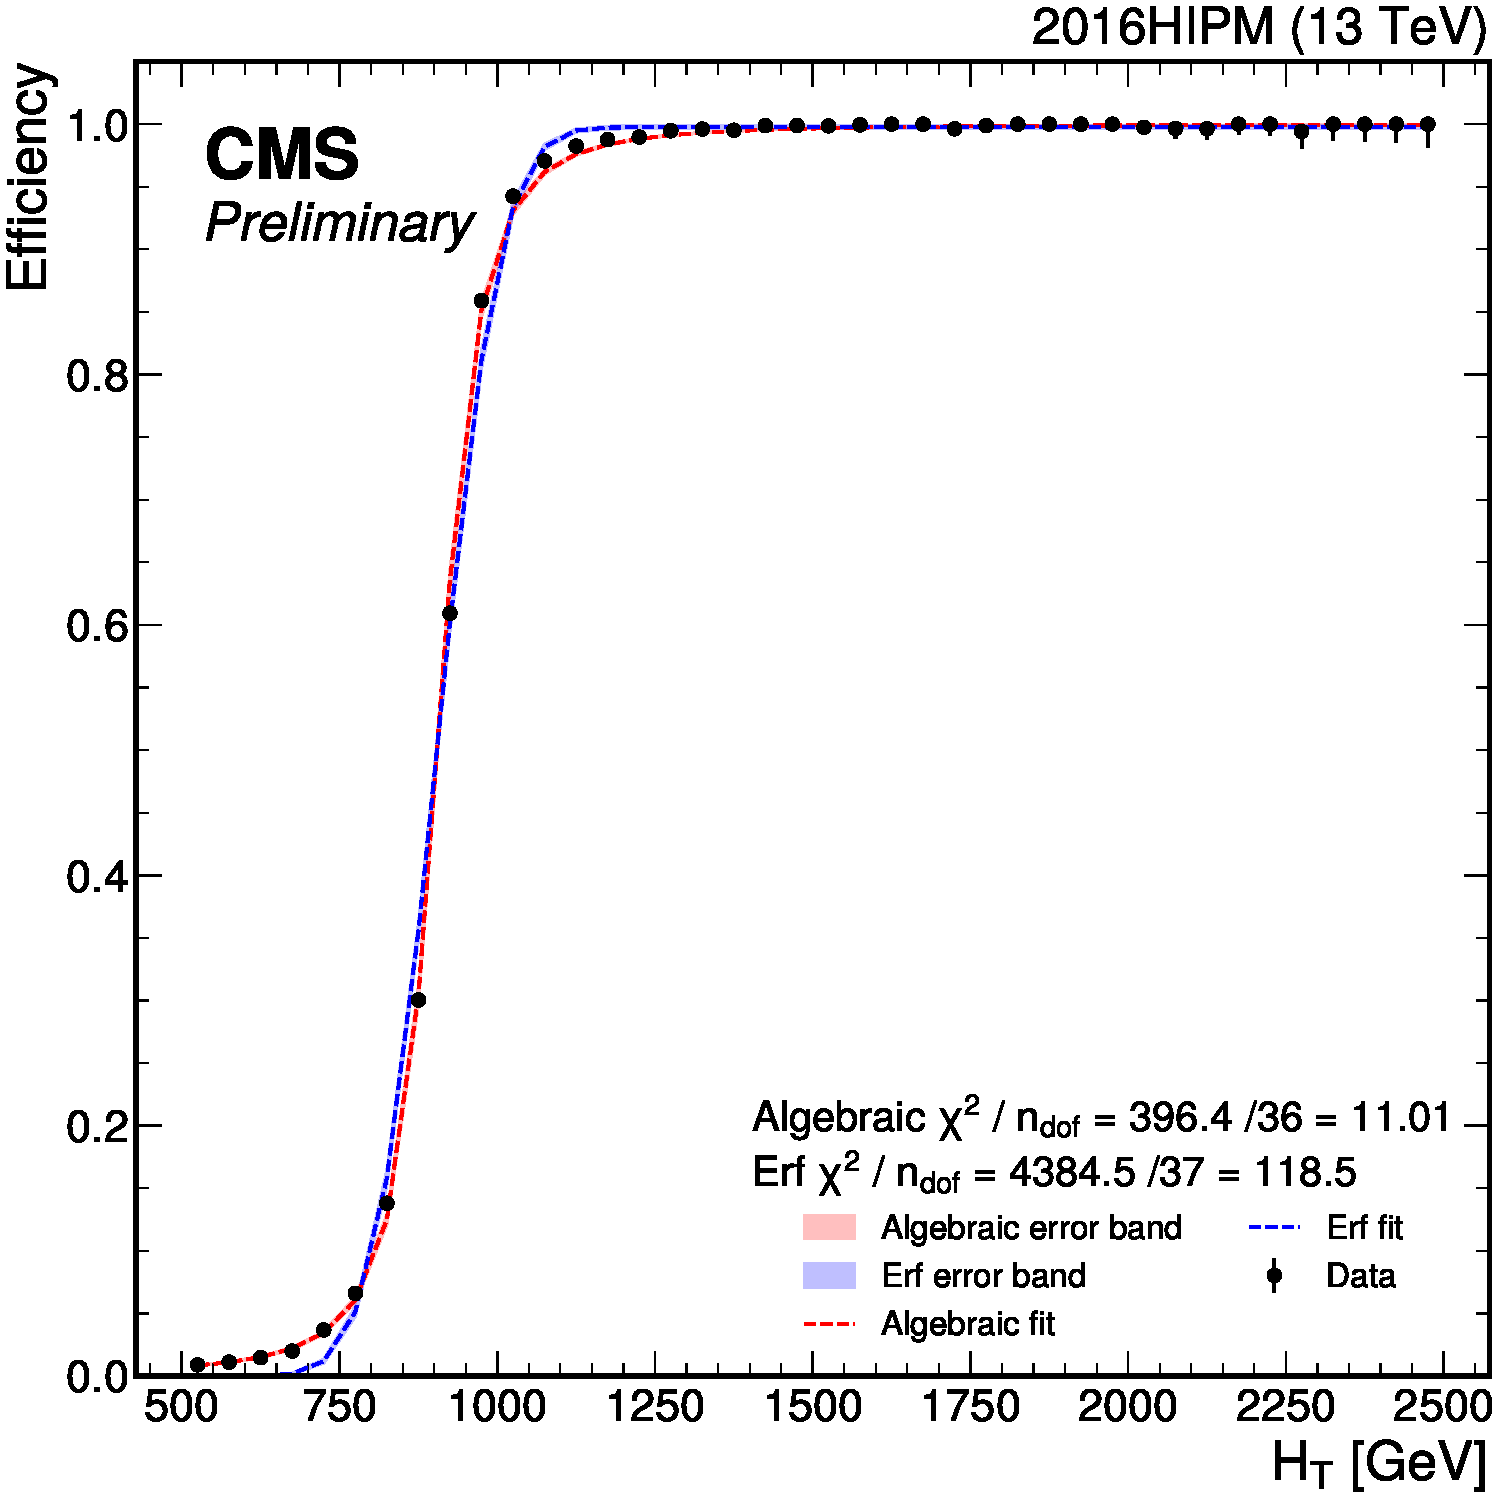
\includegraphics[width=\linewidth]{Images/pdfs/fits_16-APV-HIPM.pdf}
		% \caption{Caption}
		% \label{fig:enter-label}
	\end{subfigure}%
	\begin{subfigure}{.36\linewidth}
		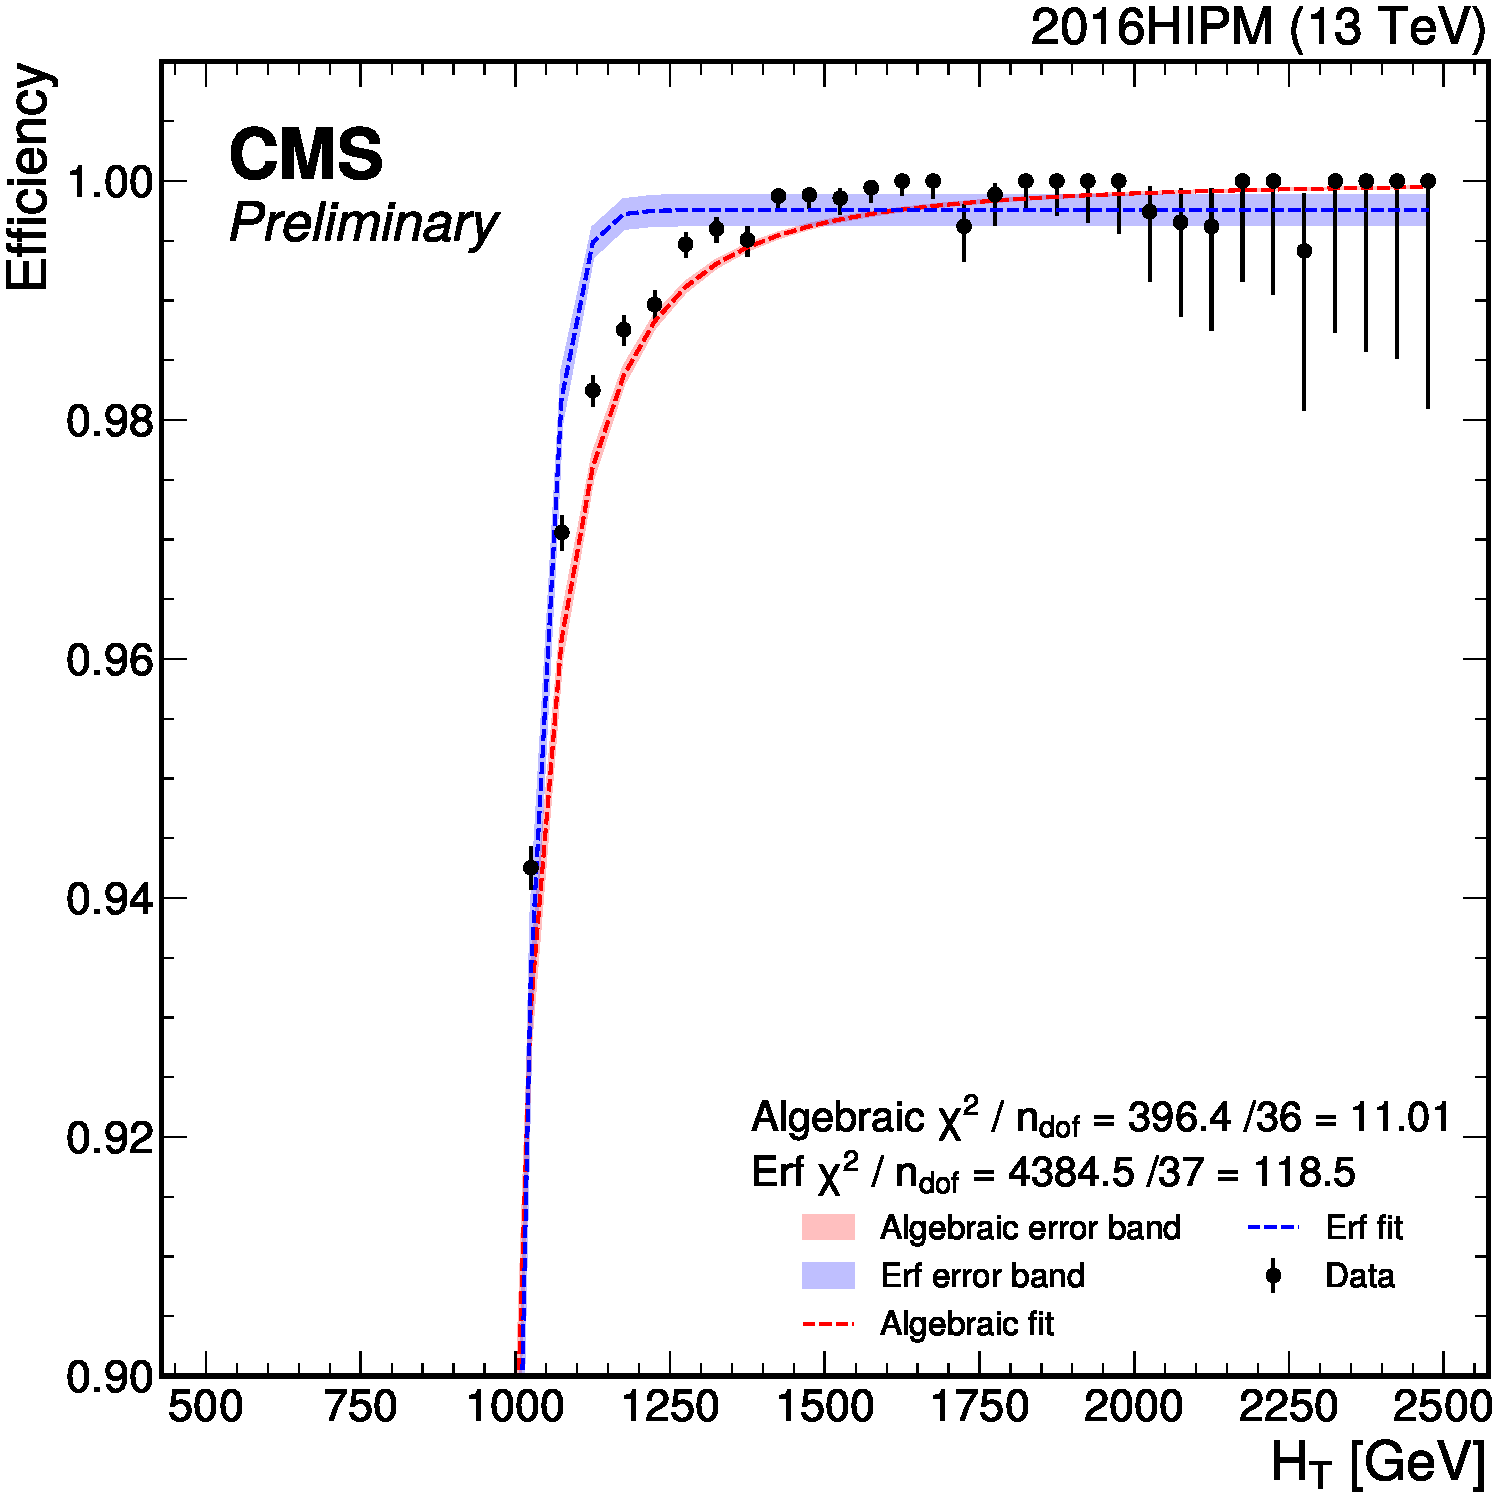
\includegraphics[width=\linewidth]{Images/pdfs/fits_closeup_16-APV-HIPM.pdf}
		% \caption{Caption}
		% \label{fig:enter-label}
	\end{subfigure}
	\begin{subfigure}{.36\linewidth}
		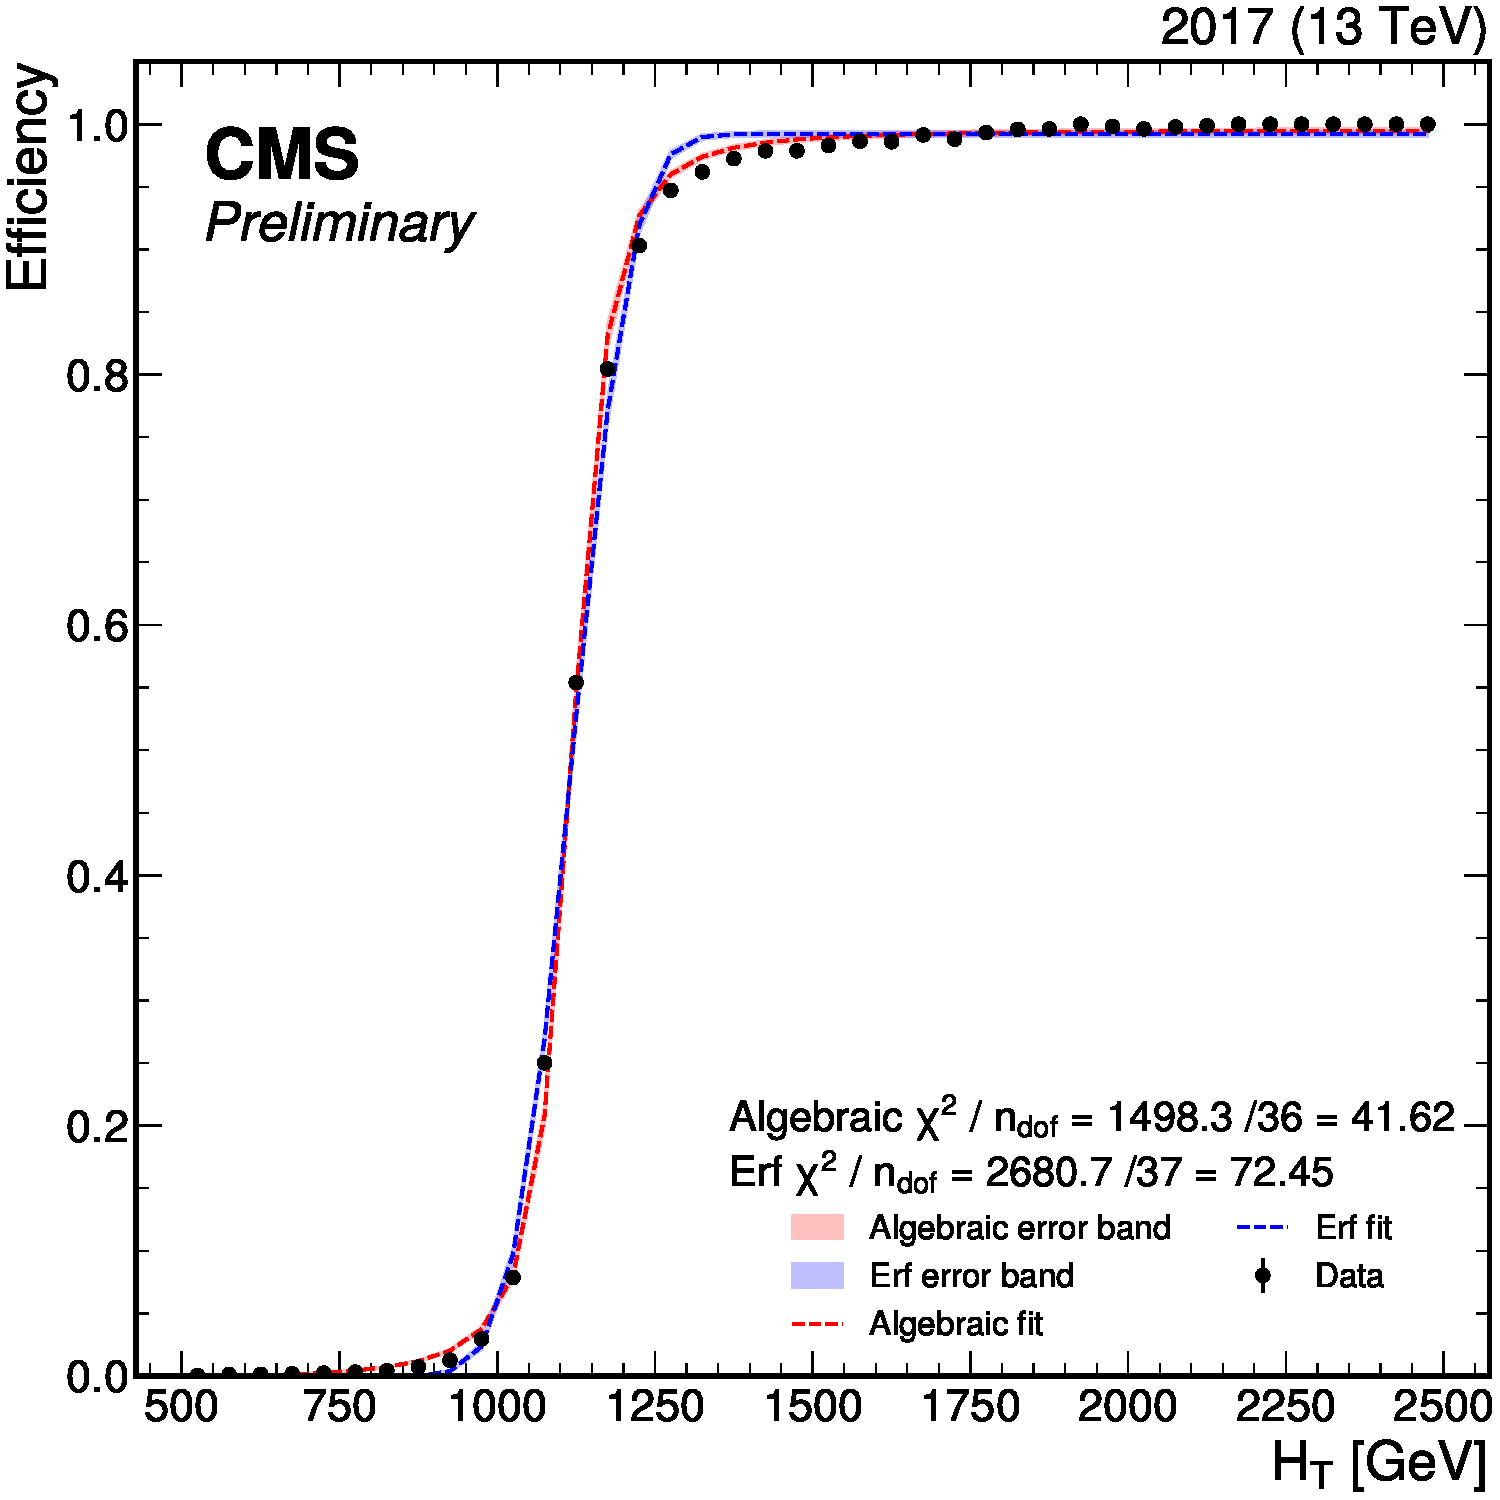
\includegraphics[width=\linewidth]{Images/pdfs/fits_17.pdf}
		% \caption{Caption}
		% \label{fig:enter-label}
	\end{subfigure}%
	\begin{subfigure}{.36\linewidth}
		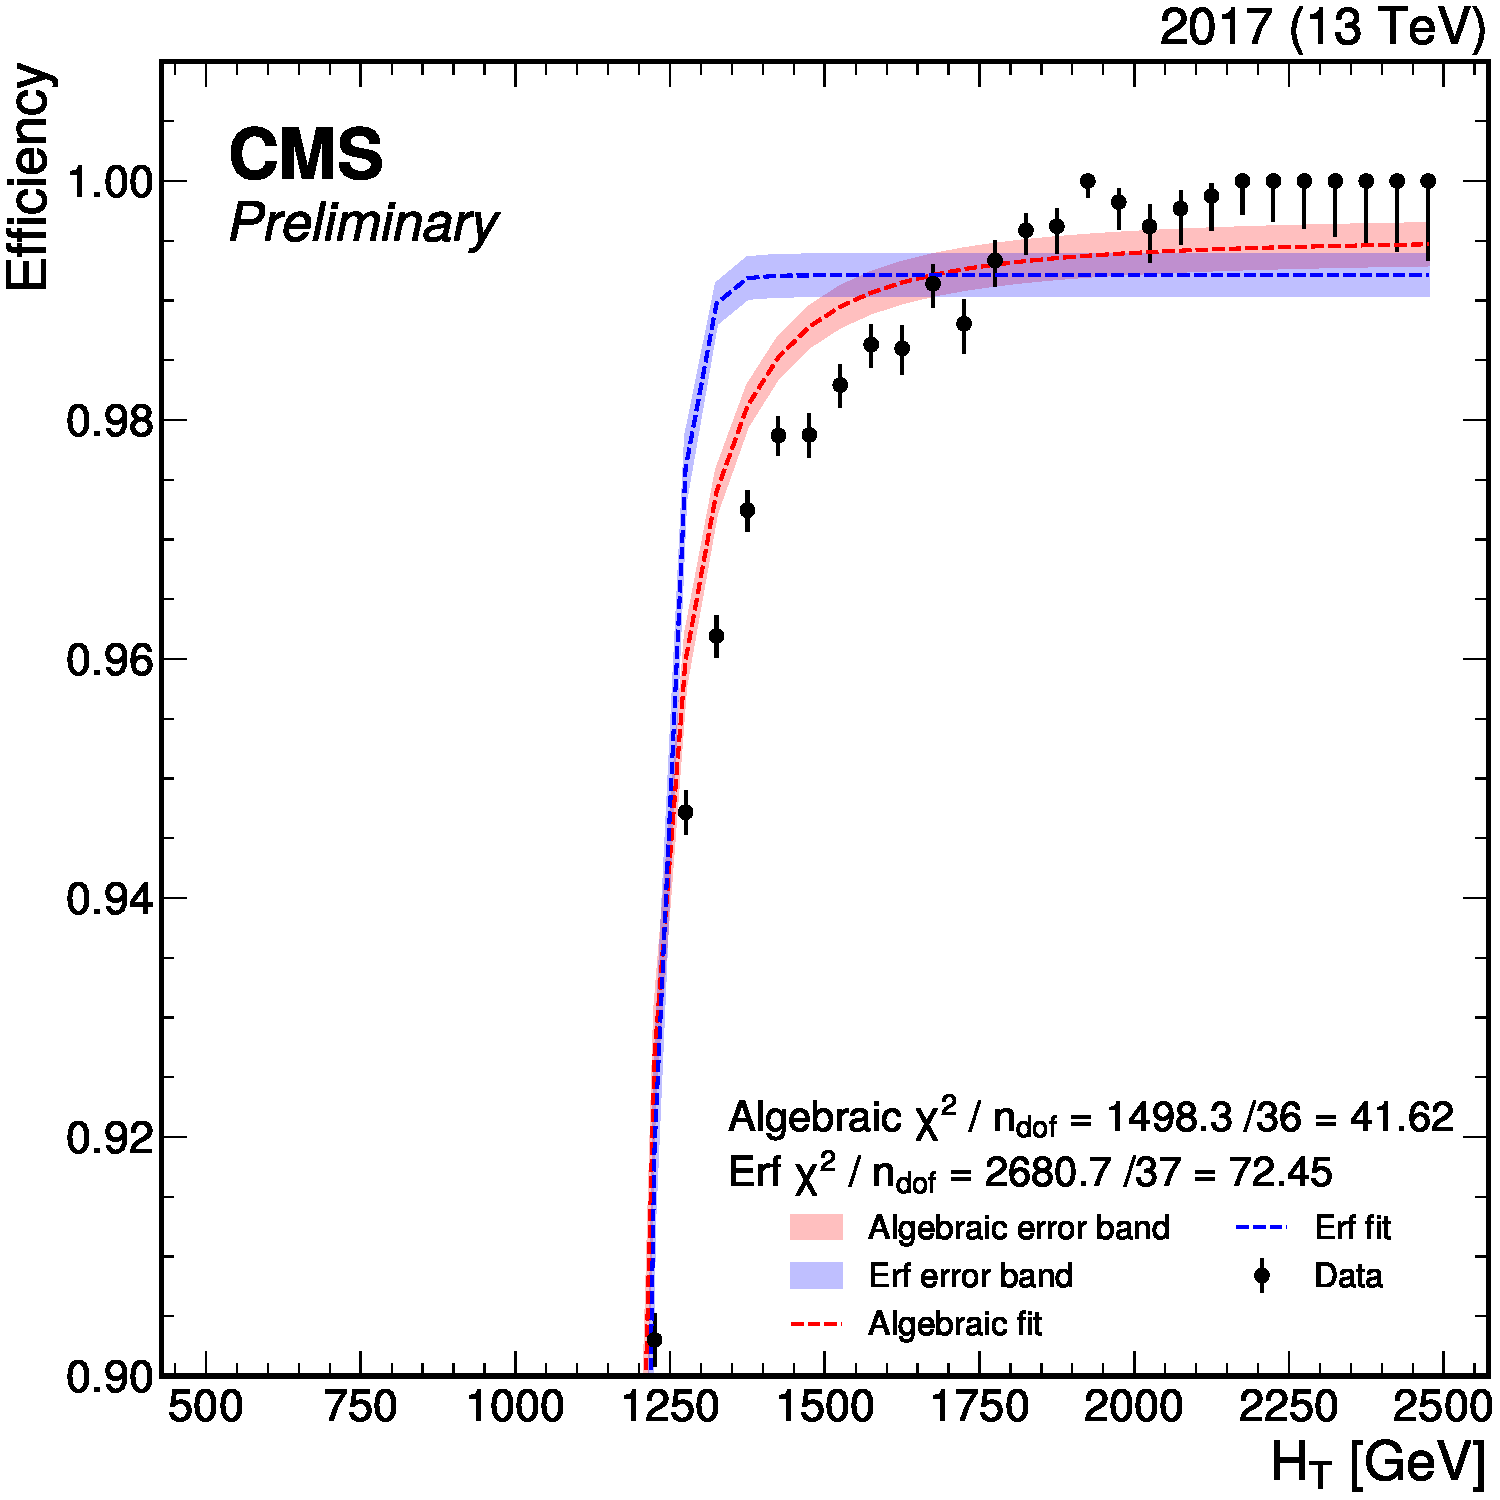
\includegraphics[width=\linewidth]{Images/pdfs/fits_closeup_17.pdf}
		% \caption{Caption}
		% \label{fig:enter-label}
	\end{subfigure}
	\begin{subfigure}{.36\linewidth}
		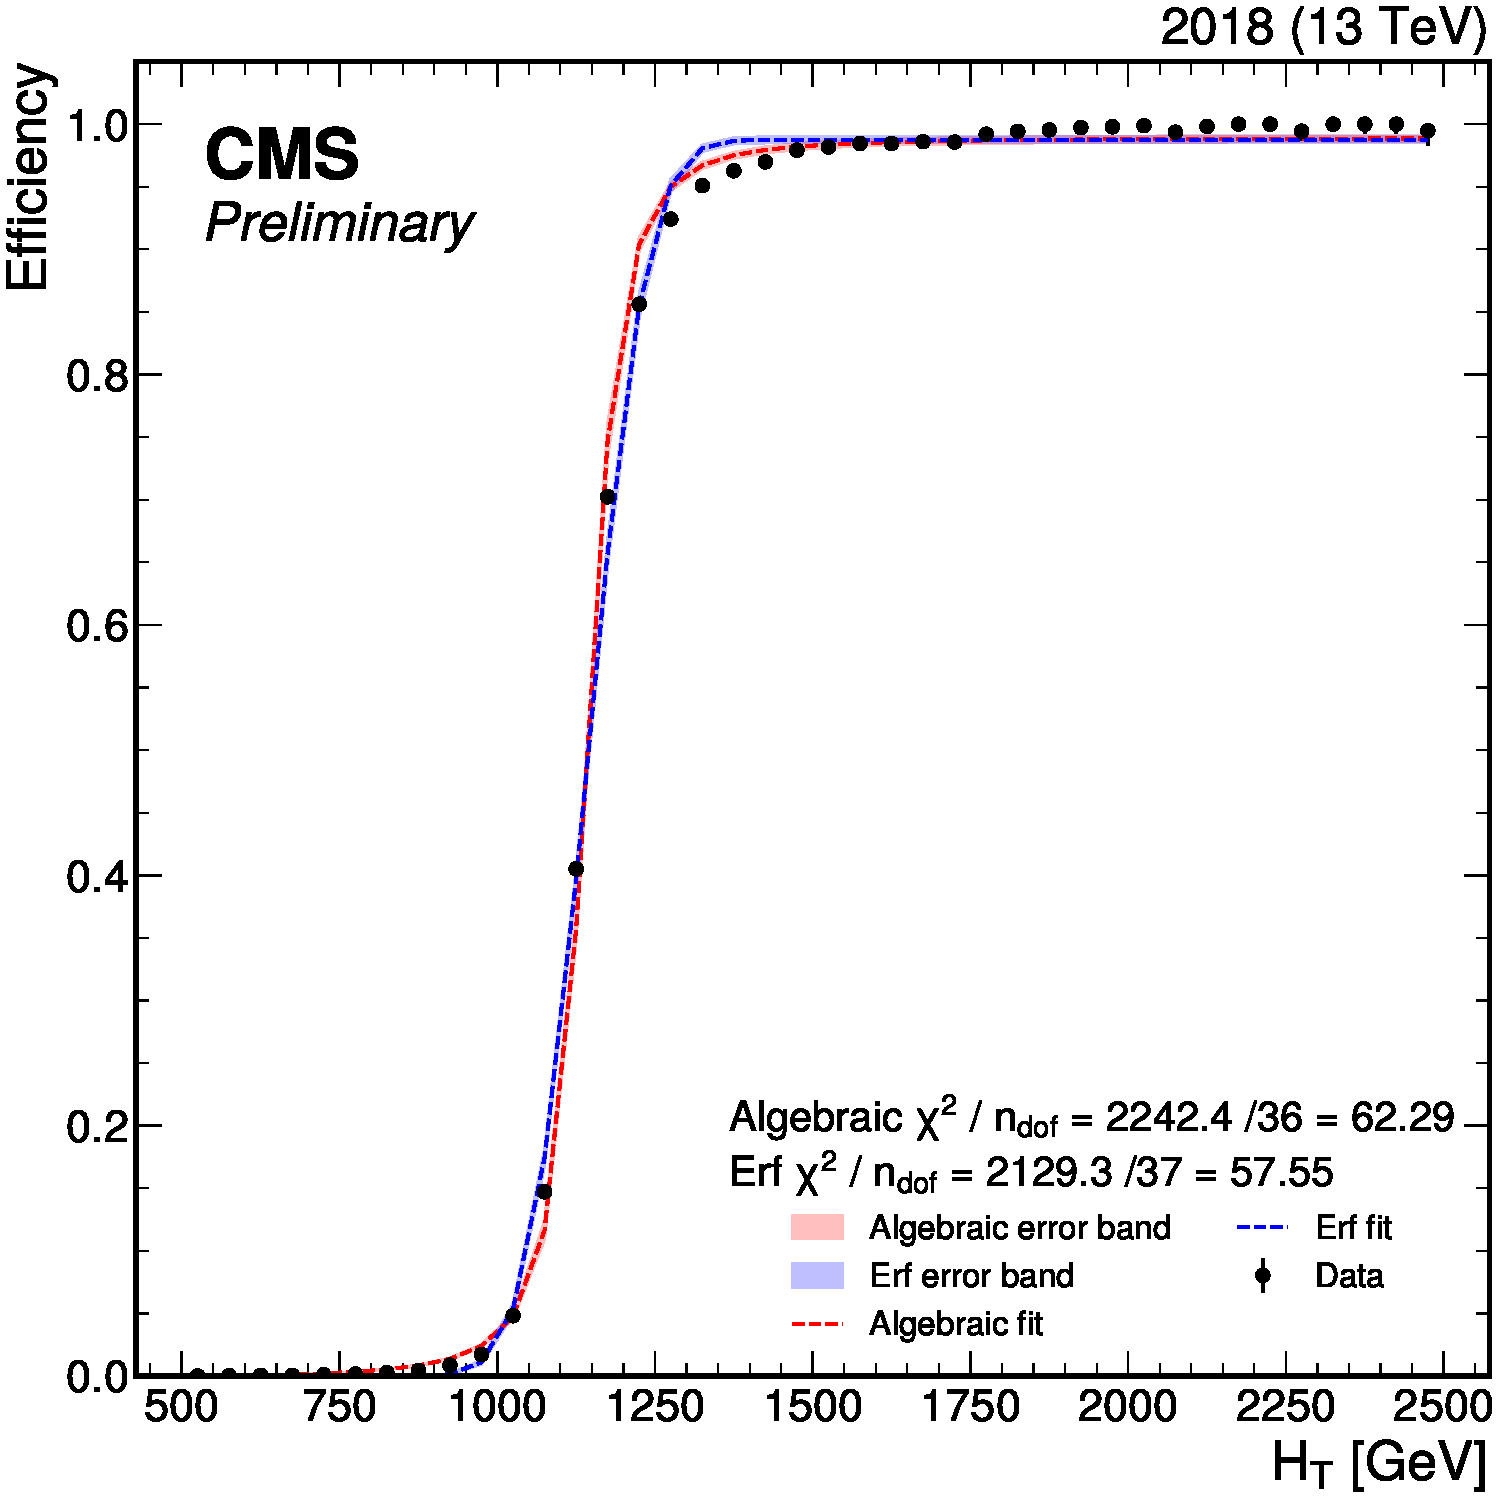
\includegraphics[width=\linewidth]{Images/pdfs/fits_18.pdf}
		% \caption{Caption}
		% \label{fig:enter-label}
	\end{subfigure}%
	\begin{subfigure}{.36\linewidth}
		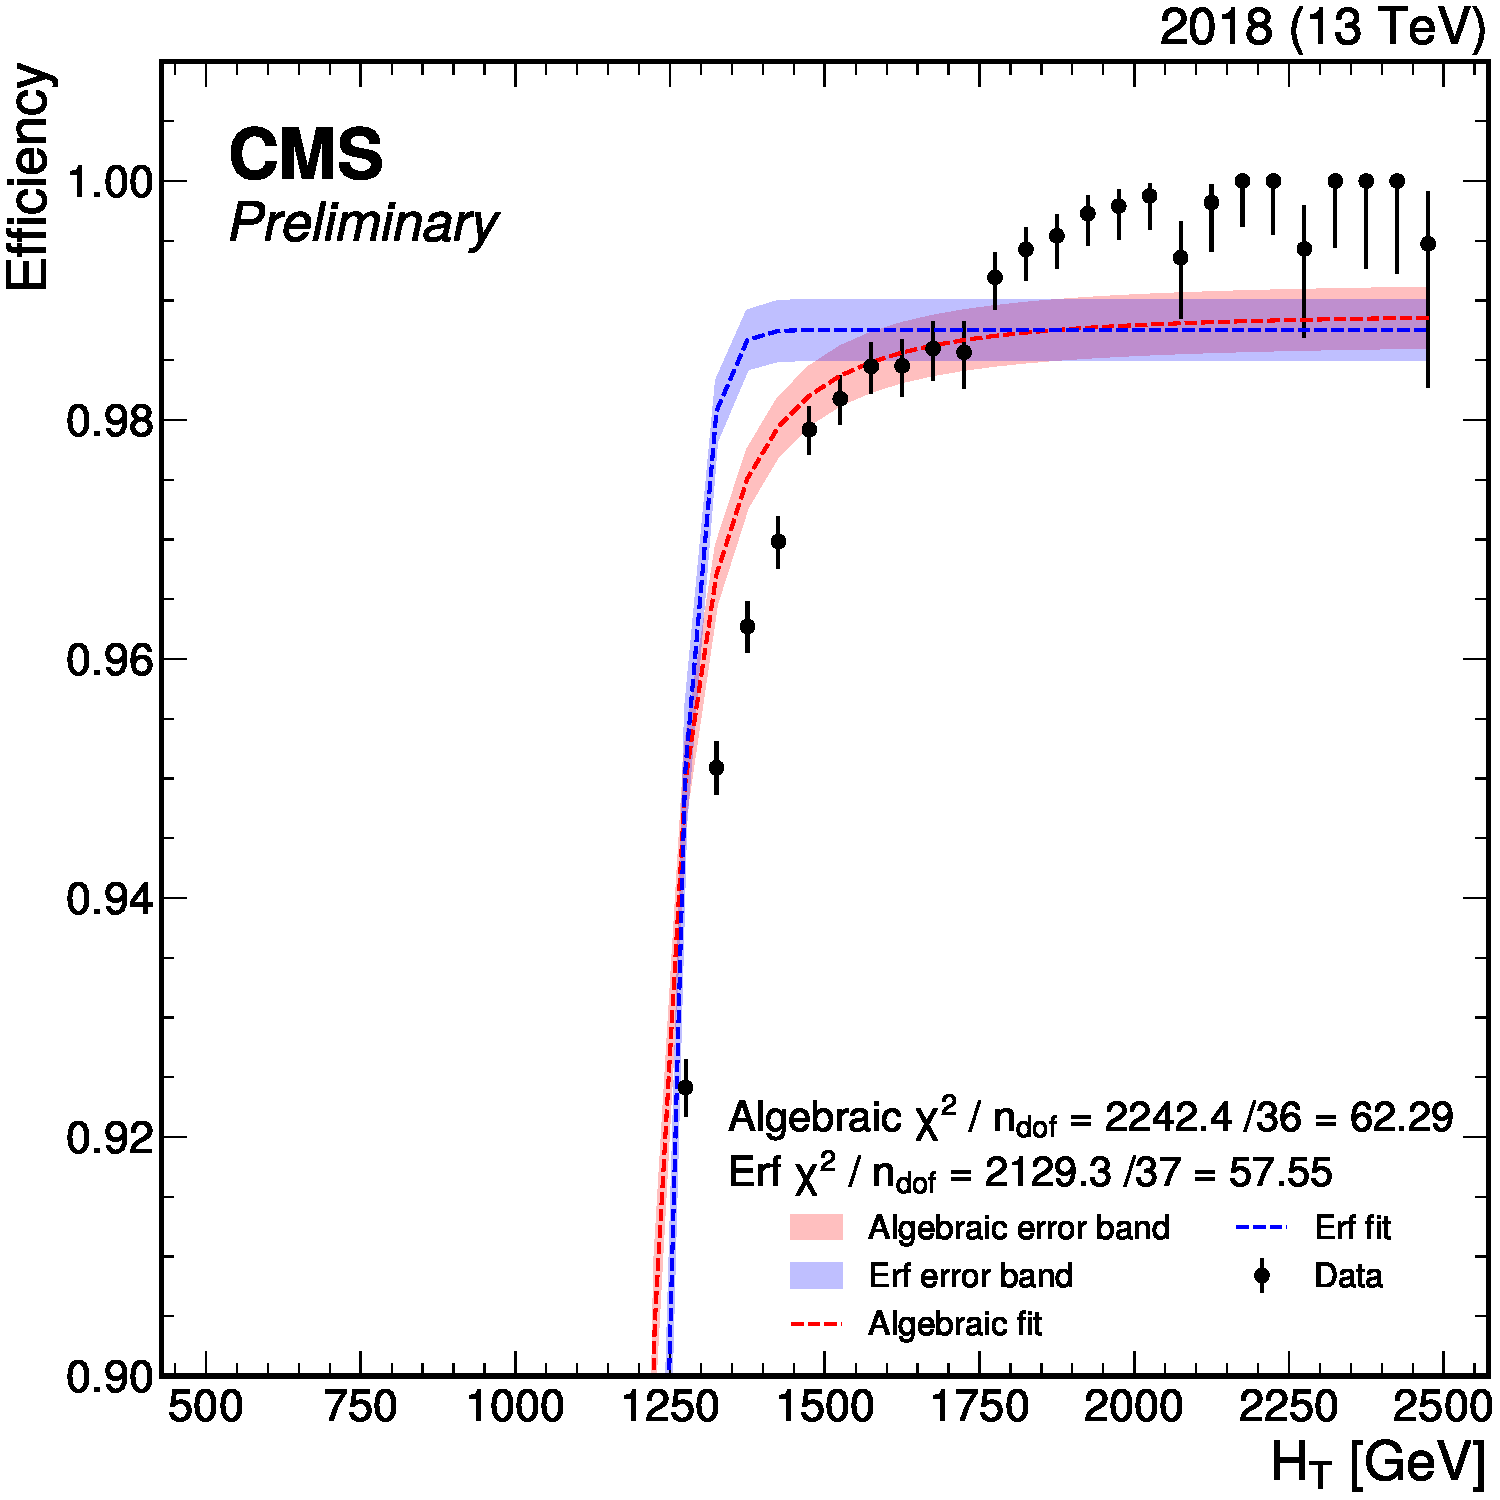
\includegraphics[width=\linewidth]{Images/pdfs/fits_closeup_18.pdf}
		% \caption{Caption}
		% \label{fig:enter-label}
	\end{subfigure}
	\caption{More detailed plots that show information about the goodness-of-fit, namely de $\chi^2$ statistic.}
	\label{fig:fits}
\end{figure}

\clearpage
